\documentclass[10pt,twocolumn]{article}
\usepackage[utf8]{inputenc}
\usepackage[T1]{fontenc}
\usepackage{lmodern}
\usepackage[activate={true,nocompatibility},final,tracking=true,kerning=true,spacing=true]{microtype}
\usepackage[letterpaper,top=0.68in,bottom=0.68in,left=0.60in,right=0.60in]{geometry}
\usepackage{amsmath,amssymb}
\usepackage{booktabs}
\usepackage{graphicx}
\usepackage{xcolor}
\usepackage{array}
\usepackage{caption}
\usepackage{enumitem}
\usepackage{fancyhdr}
\usepackage{titlesec}
\usepackage{hyperref}

\definecolor{navyaccent}{RGB}{18,54,99}
\definecolor{slateborder}{RGB}{195,205,218}
\definecolor{abstractbg}{RGB}{247,249,252}

\hypersetup{
    colorlinks=true,
    linkcolor=navyaccent,
    citecolor=navyaccent,
    urlcolor=navyaccent,
    pdftitle={MedTRT: Eliminating End-to-End I/O, 3D Affine Resampling, and FP16 Quantization Bottlenecks in Volumetric CT Organ Segmentation},
    pdfauthor={Diego Diaz Rivera},
    pdfsubject={Biomedical AI Systems, Custom CUDA C++17 Kernels, and TensorRT FP16 Numerical Validation},
    pdfkeywords={3D CT Segmentation, 3D Residual U-Net, MONAI, CUDA C++17, TensorRT, FP16 Quantization, BatchNorm Folding, Amdahl's Law, TOST Equivalence}
}

\setlength{\columnsep}{0.22in}
\setlength{\emergencystretch}{1.6em}
\captionsetup{font=footnotesize,labelfont={bf,color=navyaccent},skip=4pt}
\setlist{nosep,leftmargin=1.35em}

\titleformat{\section}{\large\bfseries\color{navyaccent}}{\thesection.}{0.5em}{}
\titlespacing*{\section}{0pt}{8pt plus 2pt minus 2pt}{4pt}
\titleformat{\subsection}{\normalsize\bfseries}{\thesubsection}{0.5em}{}
\titlespacing*{\subsection}{0pt}{6pt plus 2pt minus 1pt}{2.5pt}

\pagestyle{fancy}
\fancyhf{}
\fancyhead[L]{\footnotesize\textit{MedTRT: End-to-End GPU Systems \& FP16 Numerical Equivalence in Volumetric 3D CT Segmentation}}
\fancyhead[R]{\footnotesize\textit{D.\ D\'iaz Rivera (2026)}}
\fancyfoot[C]{\footnotesize\thepage}
\renewcommand{\headrulewidth}{0.4pt}
\fancypagestyle{plain}{
    \fancyhf{}
    \fancyfoot[C]{\footnotesize\thepage}
    \renewcommand{\headrulewidth}{0pt}
}

\renewcommand{\topfraction}{0.95}
\renewcommand{\bottomfraction}{0.95}
\renewcommand{\dbltopfraction}{0.95}
\renewcommand{\textfraction}{0.04}
\renewcommand{\floatpagefraction}{0.88}
\renewcommand{\dblfloatpagefraction}{0.88}
\setcounter{topnumber}{4}
\setcounter{bottomnumber}{4}
\setcounter{totalnumber}{8}
\setcounter{dbltopnumber}{4}
\setlength{\textfloatsep}{6pt plus 2pt minus 2pt}
\setlength{\dbltextfloatsep}{6pt plus 2pt minus 2pt}

\begin{document}

\twocolumn[{%
\begin{@twocolumnfalse}
\begin{center}
    {\LARGE\bfseries\color{navyaccent} MedTRT: Eliminating End-to-End I/O, 3D Affine Resampling, and FP16 Quantization Bottlenecks in Volumetric CT Organ Segmentation\par}
    \vspace{6pt}
    {\normalsize\bfseries Diego D\'iaz Rivera\par}
    \vspace{2pt}
    {\small Department of Bioengineering, Rice University, Houston, TX, USA\\
    Biomedical AI Systems \& GPU Performance Engineering $\cdot$ \url{https://github.com/DDR9/MedTRT}\par}
    \vspace{2pt}
    {\footnotesize Technical Manuscript $\cdot$ November 2026 $\cdot$ Reproducible Artifact Fingerprint: \texttt{e9d4f060aaf1b130}\par}
\end{center}
\vspace{4pt}
\noindent\fcolorbox{slateborder}{abstractbg}{%
\begin{minipage}{\dimexpr\textwidth-2\fboxsep-2\fboxrule\relax}
\vspace{3pt}
\footnotesize
\noindent\textbf{\color{navyaccent}Abstract.}
\textbf{Background:} Three-dimensional convolutional neural networks such as the 3D Residual U-Net enable automated volumetric organ segmentation in abdominal computed tomography (CT). Processing full diagnostic volumes ($512 \times 512 \times 31\text{--}168$ voxels, $8.13 \times 10^6$ to $4.40 \times 10^7$ voxels per scan) with anisotropic physical spacing ($1.5\text{--}8.0\text{ mm}$ axial slice thickness) requires a sequential pipeline spanning file decompression, canonical coordinate reorientation, trilinear spatial resampling, overlapping sliding-window patch inference, and inverse spatial resampling to native patient geometry.
\textbf{Problem:} Profiling the pretrained MONAI \texttt{spleen\_ct\_segmentation} v0.6.1 bundle across \textbf{53 abdominal 3D CT volumes} ($41$ Medical Segmentation Decathlon \texttt{Task09\_Spleen} scans plus $12$ unseen external multi-center MICCAI \texttt{FLARE22} scans) on an NVIDIA GeForce RTX 5080 Laptop GPU (Blackwell \texttt{sm\_120}, $16\text{ GB}$ GDDR7) exposes three bottlenecks that defeat standalone network compilation: (1) in the baseline host pipeline (\texttt{pytorch\_fp32}, $2,952.0\text{ ms}$ median end-to-end latency), the 3D U-Net forward pass (\texttt{sw\_network} $= 254.6\text{ ms}$) consumes only $8.62\%$ of total runtime, while $91.38\%$ is spent in CPU inverse resampling ($1,990.4\text{ ms}$), \texttt{.nii.gz} decompression ($424.7\text{ ms}$), and CPU preprocessing ($286.4\text{ ms}$), bounding theoretical network-only speedup via Amdahl's Law to $S_{\max} = 1.094\times$; (2) moving spatial transforms onto the GPU via MONAI's \texttt{SpatialResample} backend (\texttt{trt\_fp16\_gpu}, $215.5\text{ ms}$) promotes 3D homogeneous coordinates to \texttt{torch.float64} and materializes dense $(1, D, H, W, 3)$ coordinate meshgrids, inflating peak allocated VRAM to \textbf{2,301 MB}; and (3) compiling the standard ONNX graph into TensorRT 10.16 FP16 (\texttt{trt\_fp16\_unfolded}) induces a systematic volumetric dilation of $+1.6754 \pm 0.5531\text{ cm}^3$ across $9/9$ internal MSD scans ($p < 0.0001$) and $+1.5366 \pm 0.7680\text{ cm}^3$ across $12/12$ external \texttt{FLARE22} scans ($+1.5961 \pm 0.6721\text{ cm}^3$ across all $21/21$ pooled patients) because PyTorch's ONNX exporter leaves decoder \texttt{ConvTranspose3d+BatchNorm3d} blocks unfused, exposing a $-81.79$ shift in \texttt{model.2.0.adn.N} where binary16 $\text{ULP}_{[64, 128)} = 0.0625$.
\textbf{Methods:} Without retraining or altering model weights semantically, we introduce: (i) analytical IEEE-754 \texttt{float64} weight folding (\texttt{fold\_conv\_transpose\_batchnorm}) prior to ONNX export; (ii) \textbf{nine custom CUDA C++17 kernels} (\texttt{cuda/medical\_kernels.cu}) that compute $3 \times 4$ voxel-to-voxel affine coordinates in scalar registers, fuse Hounsfield Unit (HU) windowing with trilinear preprocessing, and exploit binary Softmax convexity ($p_0 + p_1 = 1$) for single-channel inverse trilinear resampling, thresholding, and warp-ballot (\texttt{\_\_ballot\_sync}) foreground counting; and (iii) zero-copy TensorRT 10.16 execution paired with OS page-cached \texttt{.nii} memory mapping (\texttt{mmap}), an interactive 3D tri-planar verification workstation, 66 automated \texttt{pytest} tests, and 14 deterministic offline claim checks.
\textbf{Results:} At matched sliding windows ($\text{overlap}=0.5, B=4$), our controlled pipeline (\texttt{trt\_fp16\_cuda}) lowers median latency from $2,952.0\text{ ms}$ to \textbf{96.3 ms} (\textbf{30.67$\times$} cohort median speedup; \textbf{33.14$\times$} paired patient-level mean speedup, $95\%$ CI $[27.61\times, 38.67\times]$) and cuts peak VRAM from $2,301\text{ MB}$ to \textbf{455 MB} (\textbf{5.06$\times$} reduction). Our fast-window operating point (\texttt{trt\_fp16\_optimized}, $\text{overlap}=0.25, B=8$) reaches \textbf{68.9 ms} median latency (\textbf{42.86$\times$} cohort speedup; \textbf{46.64$\times$} paired median speedup; $87.44\text{ ms}$ median across all 41 MSD volumes). Analytical FP64 folding reduces mean absolute logit drift by \textbf{35.6$\times$} ($0.1377 \to 0.00387$) and satisfies paired Two One-Sided Tests (TOST) equivalence against strict IEEE FP32 within $\Delta_V = \pm 0.10\text{ cm}^3$ across internal MSD ($+0.0010 \pm 0.0194\text{ cm}^3$, $p_{\text{TOST}} < 10^{-6}$), external \texttt{FLARE22} ($-0.0110 \pm 0.0315\text{ cm}^3$, $p_{\text{TOST}} < 10^{-6}$), and pooled $N = 21$ patients ($-0.0059 \pm 0.0271\text{ cm}^3$, $90\%$ CI $[-0.0161, +0.0043]\text{ cm}^3$, $p_{\text{TOST}} < 10^{-6}$), maintaining Mean Dice $0.9652$, $\max |\Delta\text{Dice}| = 0.000029$, Mean $\text{HD}_{95} = 2.18\text{ mm}$, and Mean $\text{ASSD} = 0.39\text{ mm}$.
\textbf{Conclusion:} Real-time, numerically faithful 3D medical segmentation requires co-designing storage ingestion, register-level GPU spatial kernels, and pre-export algebraic conditioning alongside neural network compilation.\\[3pt]
\noindent\textbf{\color{navyaccent}Index Terms:} 3D Computed Tomography, Volumetric Organ Segmentation, CUDA C++17, NVIDIA TensorRT, FP16 Quantization, Transposed Convolution BatchNorm Folding, Amdahl's Law, Quantitative Volumetry, TOST Equivalence.\\[2pt]
\noindent\textit{Research Disclosure: MedTRT is an educational and scientific GPU systems benchmark on public retrospective datasets and is not a cleared clinical medical device.}
\vspace{2pt}
\end{minipage}%
}
\vspace{10pt}
\end{@twocolumnfalse}%
}]

\section{Introduction}
\label{sec:intro}

Three-dimensional convolutional neural networks (3D CNNs), led by the 3D U-Net \cite{cicek2016} and 3D Residual U-Net \cite{kerfoot2019}, serve as standard architectures in computational biomedical imaging for automated organ segmentation in abdominal computed tomography (CT). Quantitative volumetric measurements derived from 3D CT segmentation support research workflows in splenomegaly tracking for portal hypertension and hematologic disorders, organ-at-risk delineation in radiation oncology, trauma volumetry, and computer-assisted surgical modeling. Deploying 3D volumetric segmentation pipelines at interactive latencies nevertheless poses computational and numerical challenges that differ fundamentally from two-dimensional natural image inference.

Whereas a standard 2D RGB image ($224 \times 224 \times 3$) contains $1.5 \times 10^5$ scalar values on an isotropic pixel lattice, a diagnostic abdominal 3D CT scan contains $512 \times 512 \times Z$ voxels, where $Z$ (axial slice count, dimensionless integer in $[31, 168]$) yields $8.13 \times 10^6$ to $4.40 \times 10^7$ voxels per volume in our 53-scan evaluation. Each CT volume is embedded in physical patient coordinates (millimeters) via a homogeneous affine matrix $A \in \mathbb{R}^{4 \times 4}$ with pronounced axial anisotropy ($0.59\text{--}0.98\text{ mm}$ in-plane pixel spacing vs.\ $1.5\text{--}8.0\text{ mm}$ slice thickness). Because evaluating a 3D CNN monolithically across $4.4 \times 10^7$ voxels exceeds standard GPU activation memory, medical imaging frameworks such as MONAI \cite{cardoso2022,monaibundle2024} execute a multi-stage volumetric pipeline: decompressing NIfTI files, reorienting scanner axes to canonical Right-Anterior-Superior (\texttt{RAS}) orientation, resampling voxel spacing to a canonical lattice ($1.5 \times 1.5 \times 2.0\text{ mm}$), running Gaussian-weighted sliding-window inference over $96 \times 96 \times 96$ patches, and inverting the predicted probability field back to native patient geometry.

Conventional deep learning deployment studies focus primarily on accelerating neural network layers using reduced-precision graph compilers such as NVIDIA TensorRT \cite{tensorrt2025}. In this paper, we demonstrate that accelerating the neural network in isolation fails both computationally and numerically on volumetric 3D CT segmentation. First, when non-network stages consume $91.38\%$ of end-to-end execution time, Amdahl's Law \cite{amdahl1967} restricts total pipeline speedup below $1.095\times$ even for an infinitely fast neural network. Second, migrating spatial transforms onto the GPU via standard framework primitives triggers a $2,301\text{ MB}$ VRAM spike caused by silent \texttt{torch.float64} promotion and dense 3D coordinate meshgrid materialization. Third, compiling unmodified ONNX exports into IEEE-754 half precision (\texttt{FP16}) introduces a systematic $+1.60\text{ cm}^3$ volumetric organ dilation across $21/21$ internal and external CT scans due to unfused decoder transposed-convolution batch normalization.

This report presents the complete architecture, mathematical derivations, kernel implementations, software verification infrastructure, and multi-cohort experimental validation of \textbf{MedTRT}, an end-to-end GPU systems and numerical-fidelity platform built around a pretrained MONAI 3D Residual U-Net (\texttt{spleen\_ct\_segmentation} v0.6.1 \cite{monaibundle2024,xia2018}) and evaluated across 53 abdominal CT volumes from the Medical Segmentation Decathlon (\texttt{Task09\_Spleen}) \cite{antonelli2022,simpson2019} and the unseen external multi-center MICCAI \texttt{FLARE22} benchmark \cite{ma2023flare}.

\section{Background: The Five Stages of Volumetric 3D CT Segmentation}
\label{sec:background}

To establish exact mathematical notation across high-performance GPU computing, numerical analysis, and biomedical image analysis, we formalize the five sequential stages of volumetric CT organ segmentation.

\subsection{Stage 1: CT Attenuation Physics and NIfTI Ingestion}
Computed tomography reconstructs spatial maps of linear X-ray attenuation coefficients $\mu(x,y,z)$ (attenuation per unit path length, $\text{cm}^{-1}$), calibrated to the standardized Hounsfield Unit ($\text{HU}$, dimensionless radiodensity scale) relative to distilled water ($\mu_{\text{water}}$) and air ($\mu_{\text{air}} \approx 0$):
\begin{equation}
    \text{HU}(x, y, z) = 1000 \times \frac{\mu(x, y, z) - \mu_{\text{water}}}{\mu_{\text{water}} - \mu_{\text{air}}}
    \label{eq:hu}
\end{equation}
Under Eq.~\eqref{eq:hu}, air equals $-1000\text{ HU}$, water equals $0\text{ HU}$, splenic parenchyma spans $+35\text{ to }+65\text{ HU}$ (clamped to the abdominal soft-tissue window $[a_{\min}, a_{\max}] = [-57, +164]\text{ HU}$), and cortical bone exceeds $+400\text{ HU}$. Research volumes are stored in NIfTI-1 format (\texttt{.nii} or gzip-compressed \texttt{.nii.gz}), comprising a $352$-byte header encoding lattice dimensions $(D_x, D_y, D_z)$, scalar datatype, and the native voxel-to-world affine matrix $A_{\text{orig}} \in \mathbb{R}^{4 \times 4}$, followed by contiguous voxel payloads ($31\text{--}168\text{ MB}$ in \texttt{float32}). Ingesting \texttt{.nii.gz} requires single-threaded CPU DEFLATE decompression prior to host-to-device (\texttt{h2d}) PCIe transfer, whereas uncompressed \texttt{.nii} payloads can be mapped directly into virtual address space via operating-system page-cached \texttt{mmap} \cite{brett2024}.

\subsection{Stage 2: Affine Coordinate Geometry, RAS Orientation, and Trilinear Resampling}
Clinical CT scanners acquire axial stacks under varying anatomical axis conventions (such as Left-Posterior-Superior \texttt{LPS} vs.\ Right-Anterior-Superior \texttt{RAS}) and heterogeneous voxel spacings $\mathbf{s}_{\text{orig}} = (s_x, s_y, s_z)$ (voxel dimensions, $\text{mm}$). Given discrete native voxel indices $\mathbf{i} = [i, j, k, 1]^T$, physical coordinates $\mathbf{p}_{\text{world}}$ (spatial position, $\text{mm}$) satisfy $\mathbf{p}_{\text{world}} = A_{\text{orig}} \mathbf{i}$. Reorienting axes to canonical \texttt{RAS} and resampling spacing to $\mathbf{s}_{\text{target}} = (1.5, 1.5, 2.0)\text{ mm}$ defines a canonical affine matrix $A_{\text{res}} \in \mathbb{R}^{4 \times 4}$ and canonical grid dimensions $(D'_x, D'_y, D'_z)$. Every canonical output voxel $\mathbf{x}_o = [x_o, y_o, z_o, 1]^T$ maps to continuous source voxel coordinates $\mathbf{x}_s = [f_x, f_y, f_z, 1]^T$ through the composite voxel-to-voxel matrix $M_{\text{pre}} \in \mathbb{R}^{4 \times 4}$:
\begin{equation}
    \mathbf{x}_s = A_{\text{orig}}^{-1} A_{\text{res}} \mathbf{x}_o = M_{\text{pre}} \mathbf{x}_o
    \label{eq:affine_composition}
\end{equation}
Scalar intensity at $\mathbf{x}_s$ is interpolated from the 8 surrounding lattice corners $(x_a, y_b, z_c) \in \{\lfloor f_x \rfloor, \lfloor f_x \rfloor + 1\} \times \{\lfloor f_y \rfloor, \lfloor f_y \rfloor + 1\} \times \{\lfloor f_z \rfloor, \lfloor f_z \rfloor + 1\}$ with fractional weights $w_x = f_x - \lfloor f_x \rfloor$, $w_y = f_y - \lfloor f_y \rfloor$, and $w_z = f_z - \lfloor f_z \rfloor$, clamped to $[-57, 164]\text{ HU}$, and linearly scaled to $[0, 1]$.

\subsection{Stage 3: 3D Residual U-Net and Gaussian Sliding-Window Inference}
The MONAI \texttt{spleen\_ct\_segmentation} v0.6.1 architecture \cite{kerfoot2019,monaibundle2024} is a 5-level encoder-decoder 3D Residual U-Net with channel widths $(16, 32, 64, 128, 256)$, BatchNorm3d normalization, PReLU activations, and 3D transposed-convolution upsampling pathways outputting 2-channel logits $(L_0, L_1)$ (unnormalized log-probabilities for background and spleen). Because resampled volumes exceed the $96 \times 96 \times 96$ network patch size, sliding-window inference partitions the grid into $N_{\text{win}}$ overlapping patches with stride $s_d = \lfloor 96(1 - \omega) \rfloor$, where $\omega \in [0, 1)$ (fractional patch overlap, dimensionless), evaluates mini-batches of size $B$ (patches per forward call), and blends patch logits $L^{(p)}$ using a separable 3D Gaussian importance kernel $G(\mathbf{r}) = \exp\big(-\frac{1}{2}\sum_{d=1}^3 (r_d / \sigma_d)^2\big)$ with relative standard deviation $\sigma = 0.125$:
\begin{equation}
    L_{\text{agg}}(\mathbf{v}) = \frac{\sum_{p \in \mathcal{P}(\mathbf{v})} G(\mathbf{v} - \mathbf{o}_p) \, L^{(p)}(\mathbf{v} - \mathbf{o}_p)}{\sum_{p \in \mathcal{P}(\mathbf{v})} G(\mathbf{v} - \mathbf{o}_p)}
    \label{eq:sw_agg}
\end{equation}
where $\mathcal{P}(\mathbf{v})$ denotes the set of patches covering canonical voxel $\mathbf{v}$ and $\mathbf{o}_p$ denotes the origin of patch $p$.

\subsection{Stage 4: Inverse Spatial Resampling and Mask Discretization}
To evaluate anatomical contours in the patient's native scanner frame, aggregated logits $L_{\text{agg}} \in \mathbb{R}^{2 \times D'_x \times D'_y \times D'_z}$ are mapped to class probabilities via Softmax, resampled back to native dimensions $(D_x, D_y, D_z)$ via $M_{\text{inv}} = A_{\text{res}}^{-1} A_{\text{orig}} = M_{\text{pre}}^{-1}$, and discretized via $\arg\max_{c \in \{0,1\}}$. Trilinearly interpolating continuous probabilities prior to thresholding preserves smooth sub-voxel organ surfaces across thick CT slices ($5.0\text{--}8.0\text{ mm}$), whereas discretizing prior to nearest-neighbor inversion introduces severe axial staircase aliasing.

\subsection{Stage 5: Physical Volumetry and Surface Distance Evaluation}
Given binary predicted mask $\hat{Y} \in \{0, 1\}^{D_x \times D_y \times D_z}$ with foreground voxel count $N_{\text{fg}} = \sum_{\mathbf{i}} \hat{Y}(\mathbf{i})$, physical organ volume $V$ (organ volume, $\text{cm}^3$) is determined by the Jacobian determinant of the $3 \times 3$ linear spatial submatrix $A_{3\times 3}$ of $A_{\text{orig}}$:
\begin{equation}
    V = \frac{N_{\text{fg}} \cdot \lvert \det(A_{3\times 3}) \rvert}{1000}\;\text{cm}^3
    \label{eq:volume}
\end{equation}
Accounting for full off-diagonal affine shear and rotation terms via $\lvert\det(A_{3\times 3})\rvert$ rather than naive header zoom products prevents geometric bias on tilted gantry acquisitions.

\section{Research Questions and Contributions}
\label{sec:questions}

This study addresses one central research question:
\begin{quote}
\textit{Can 3D volumetric medical image segmentation achieve order-of-magnitude end-to-end GPU acceleration while preserving formal statistical numerical equivalence with a strict IEEE-754 FP32 reference implementation?}
\end{quote}
We decompose this question into two coupled investigations:
\begin{itemize}
    \item \textbf{Research Problem A (Systems Performance \& Amdahl's Law):} Why does standalone neural network compilation fail to accelerate end-to-end 3D CT segmentation, and how can storage ingestion, 3D affine preprocessing, and inverse probability resampling be co-designed in custom CUDA C++17 to eliminate both CPU bottlenecks and framework GPU memory bloat?
    \item \textbf{Research Problem B (FP16 Numerical Stability):} Why does standard ONNX-to-TensorRT FP16 compilation induce a systematic $+1.60\text{ cm}^3$ volumetric organ dilation across $21/21$ CT scans, and can an exact pre-export algebraic transformation restore strict IEEE-754 FP32 equivalence without sacrificing Tensor Core throughput?
\end{itemize}

\noindent\textbf{Primary Project Contributions:}
\begin{enumerate}
    \item \textbf{Six-Stage Bottleneck Telemetry \& Amdahl's Law Proof:} We instrument all six execution stages across 13 execution profiles, demonstrating that non-network overhead accounts for $91.38\%$ of host runtime ($S_{\max} = 1.094\times$) and uncovering MONAI's promotion of 3D GPU resampling coordinates to \texttt{torch.float64} ($2,301\text{ MB}$ peak VRAM).
    \item \textbf{Nine Register-Affine Custom CUDA C++17 Kernels:} We implement and profile 9 custom CUDA kernels (\texttt{cuda/medical\_kernels.cu}) compiled via NVRTC 12.8 for Blackwell \texttt{sm\_120} that compute $3 \times 4$ affine coordinates in scalar registers and exploit binary Softmax convexity to halve postprocessing memory traffic, accelerating GPU preprocessing by $\mathbf{33.8\times}$ ($43.9\text{ ms} \to 1.27\text{ ms}$), GPU postprocessing by $\mathbf{27.1\times}$ ($71.1\text{ ms} \to 2.62\text{ ms}$, or $\mathbf{760\times}$ vs.\ CPU), and reducing peak VRAM by $\mathbf{5.06\times}$ ($2,301\text{ MB} \to 455\text{ MB}$).
    \item \textbf{Root-Cause Diagnosis \& Analytical FP64 Resolution of Decoder FP16 Cancellation:} We trace the $+1.68\text{ cm}^3$ (MSD) and $+1.54\text{ cm}^3$ (\texttt{FLARE22}) unfolded FP16 dilation to asymmetric ONNX constant folding in \texttt{model.2.0.adn.N} (unfused shift $-81.79$ at $\text{ULP}_{[64,128)} = 0.0625$) and prove that analytical \texttt{float64} weight folding cuts logit drift by $\mathbf{35.6\times}$ and achieves paired TOST equivalence ($p_{\text{TOST}} < 10^{-6}$) within $\pm 0.10\text{ cm}^3$.
    \item \textbf{Multi-Cohort 53-Volume Validation, Interactive Tri-Planar Workstation, and Automated Claim Verifier:} We validate MedTRT across 41 internal MSD scans and 12 external multi-center MICCAI \texttt{FLARE22} scans, accompanied by a Streamlit 3D radiological verification workstation (\texttt{app/workstation.py}), 66 \texttt{pytest} tests, and a 14-check offline claim audit suite (\texttt{src/medtrt/verify\_claims.py}).
\end{enumerate}

\section{Baseline Bottleneck Characterization}
\label{sec:bottlenecks}

\subsection{Amdahl's Law Across Host and GPU Execution Paths}
Let $T_{\text{E2E}} = T_{\text{non-net}} + T_{\text{net}}$ (end-to-end volume latency, $\text{ms}$) and let $p = T_{\text{net}} / T_{\text{E2E}}$ (network runtime fraction, dimensionless). By Amdahl's Law \cite{amdahl1967}, accelerating the network stage by factor $S_{\text{net}}$ yields total pipeline speedup $S(S_{\text{net}})$:
\begin{equation}
\begin{aligned}
    S(S_{\text{net}}) &= \frac{1}{(1 - p) + \frac{p}{S_{\text{net}}}}, \\
    S_{\max} &= \lim_{S_{\text{net}} \to \infty} S(S_{\text{net}}) = \frac{1}{1 - p}
\end{aligned}
\label{eq:amdahl}
\end{equation}
In the baseline host pipeline (\texttt{pytorch\_fp32}, $\omega=0.5, B=4$), cohort median latency across the 9 held-out MSD scans is $2,952.0\text{ ms}$, whereas \texttt{sw\_network} requires only $254.6\text{ ms}$ ($p = 0.0862$). Non-network stages consume $2,697.4\text{ ms}$ ($91.38\%$): CPU trilinear \texttt{Invertd} ($1,990.4\text{ ms}$, $67.4\%$), \texttt{.nii.gz} decompression ($424.7\text{ ms}$, $14.4\%$), CPU preprocessing ($286.4\text{ ms}$, $9.7\%$), and window aggregation ($8.0\text{ ms}$). Substituting TensorRT FP16 on the host path (\texttt{trt\_fp16}) accelerates \texttt{sw\_network} to $167.1\text{ ms}$, yet end-to-end latency drops only to $2,880.3\text{ ms}$ ($1.02\times$ speedup), empirically confirming the Amdahl ceiling $S_{\max} = (1 - 0.0862)^{-1} = 1.094\times$ (and $S_{\max} = 1.085\times$ in our 90-pass host reference run at $3,341.1\text{ ms}$ E2E / $260.8\text{ ms}$ network). Only after eliminating host I/O and CPU spatial resampling does the network share rise to $50.9\%$ in \texttt{trt\_fp16\_cuda}, unlocking TensorRT acceleration.

\subsection{Why Framework GPU Resampling Spikes VRAM to 2,301 MB}
Migrating \texttt{Orientationd}, \texttt{Spacingd}, and \texttt{Invertd} onto the GPU via MONAI's \texttt{SpatialResample} primitive (\texttt{trt\_fp16\_gpu}) lowers median E2E latency to $215.5\text{ ms}$, but hardware instrumentation (\texttt{src/medtrt/probes.py}) identified two severe bottlenecks:
\begin{enumerate}
    \item \textbf{Silent \texttt{torch.float64} Coordinate Promotion:} MONAI constructs 3D homogeneous voxel grids $(1, 4, D, H, W)$ in \texttt{torch.float64} on \texttt{cuda:0} prior to invoking \texttt{grid\_sample}. On consumer Blackwell GPUs (\texttt{sm\_120}), FP64 instruction throughput is $1/64$ of FP32 throughput.
    \item \textbf{Dense 3D Coordinate Meshgrid Allocation:} PyTorch's \texttt{grid\_sample} requires a materialized $(1, D, H, W, 3)$ sampling tensor in global memory. On \texttt{spleen\_6} ($512 \times 512 \times 135 = 35,389,440$ voxels), this allocates $961.4\text{ MB}$ of incremental VRAM during preprocessing and $2,100.2\text{ MB}$ during 2-channel trilinear postprocessing, pushing full-pipeline peak allocated VRAM to $\mathbf{2,301.3\textbf{ MB}}$ ($3,667.7\text{ MB}$ reserved) compared to $487\text{ MB}$ on the CPU transform path (Figure~\ref{fig:arch_diagram}).
\end{enumerate}

\begin{figure*}[t]
    \centering
    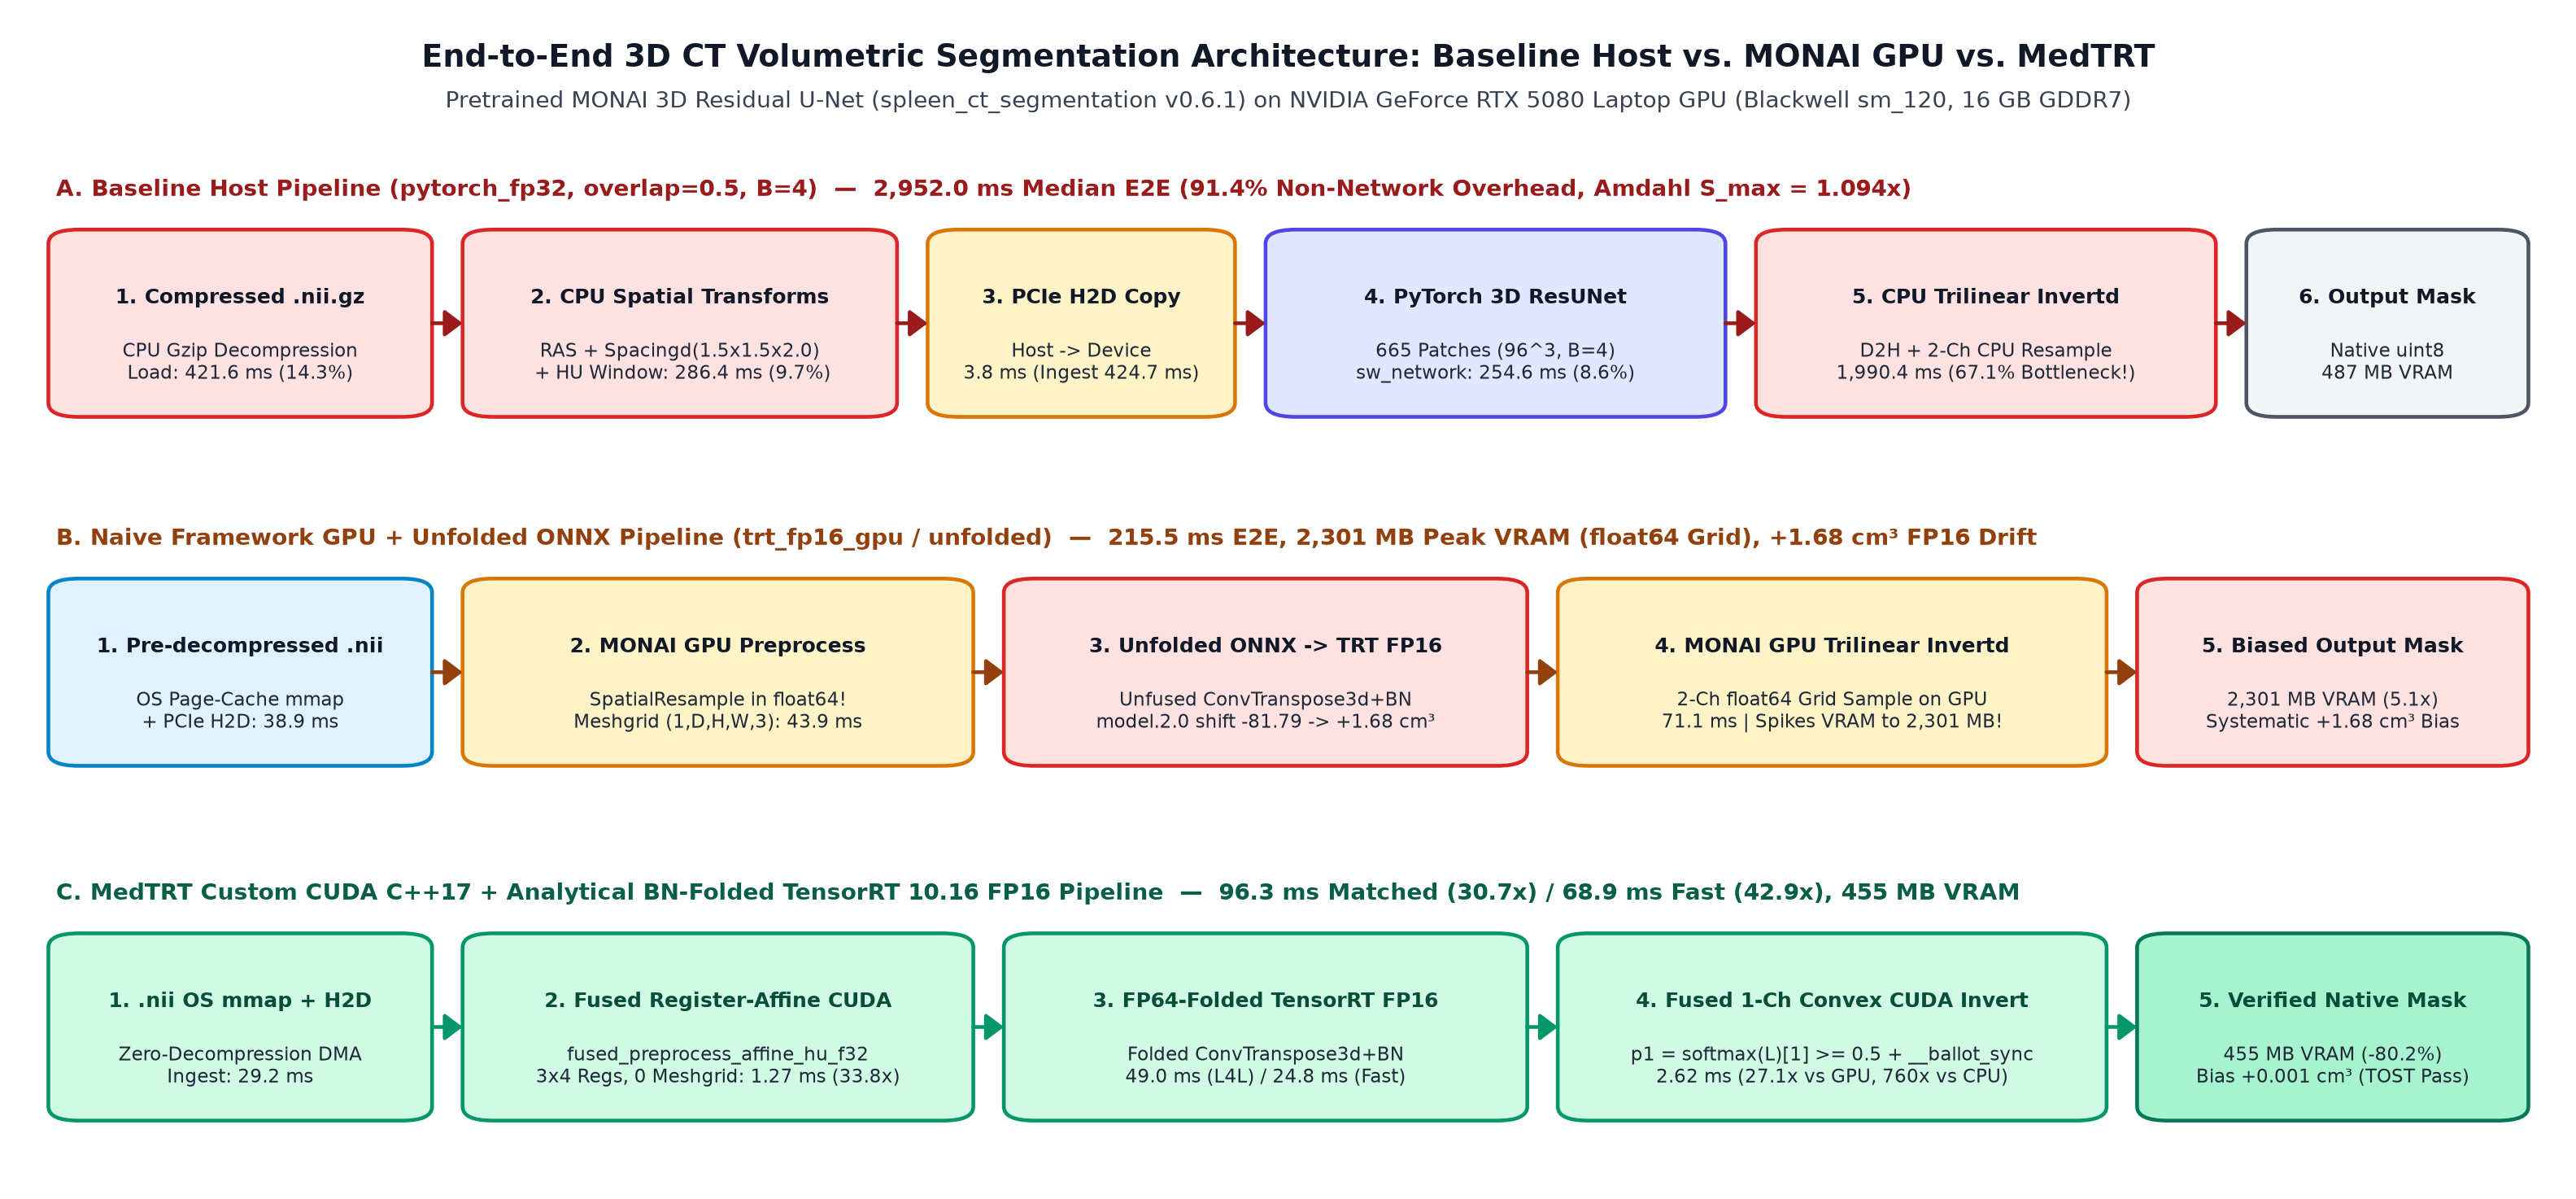
\includegraphics[width=0.93\textwidth]{figures/pipeline_architecture.png}
    \caption{End-to-end architectural comparison of (A) the Baseline Host Pipeline (\texttt{pytorch\_fp32}, $2,952.0\text{ ms}$ median E2E, $91.4\%$ non-network overhead, $S_{\max} = 1.094\times$), (B) the Framework GPU + Unfolded ONNX Pipeline (\texttt{trt\_fp16\_gpu} / \texttt{unfolded}, $215.5\text{ ms}$ E2E, $2,301\text{ MB}$ peak VRAM from \texttt{float64} coordinate meshgrids, and $+1.68\text{ cm}^3$ FP16 volume dilation), and (C) the MedTRT Custom CUDA C++17 + Analytical FP64-Folded TensorRT 10.16 Pipeline ($96.3\text{ ms}$ matched / $68.9\text{ ms}$ fast, $455\text{ MB}$ peak VRAM, $+0.001\text{ cm}^3$ internal volume bias).}
    \label{fig:arch_diagram}
\end{figure*}

\section{MedTRT System Architecture and Custom CUDA C++17 Kernels}
\label{sec:cuda}

To eliminate host CPU bottlenecks and MONAI's $2,301\text{ MB}$ coordinate meshgrids simultaneously, MedTRT implements \textbf{nine custom CUDA C++17 \texttt{\_\_global\_\_} kernels} in \texttt{cuda/medical\_kernels.cu} (Table~\ref{tab:kernels}). All kernels are compiled at runtime to native Blackwell \texttt{compute\_120} (\texttt{sm\_120}) SASS via NVRTC 12.8 (\texttt{-{}-gpu-architecture=compute\_120 -{}-use\_fast\_math -default-device}) and launched zero-copy on PyTorch device pointers (\texttt{tensor.data\_ptr()}) through the CUDA Driver API (\texttt{nvcuda.dll}).

\subsection{Register-Computed $3 \times 4$ Affine Coordinate Mapping}
Rather than allocating $(1, D, H, W, 3)$ coordinate tensors in global GDDR7 memory, we precompute the exact $3 \times 4$ voxel-to-voxel matrices $M_{\text{pre}} = (A_{\text{orig}}^{-1} A_{\text{res}})_{[0:3, 0:4]}$ and $M_{\text{inv}} = (A_{\text{res}}^{-1} A_{\text{orig}})_{[0:3, 0:4]}$ on the host in IEEE-754 \texttt{float64} (\texttt{compute\_ras\_resampled\_geometry} in \texttt{src/medtrt/cuda\_kernels.py}, matching MONAI's target affine to $4.44 \times 10^{-16}$) and pass the 12 scalar \texttt{float32} entries $(m_{00}, \dots, m_{23})$ by value in constant kernel parameter registers. Each GPU thread assigned to output voxel $(x_o, y_o, z_o)$ within an $(8 \times 8 \times 4) = 256$-thread 3D block evaluates its source coordinates $(f_x, f_y, f_z)$ directly in scalar registers via hardware fused multiply-add (\texttt{FFMA}) instructions:
\begin{equation}
\begin{bmatrix} f_x \\ f_y \\ f_z \end{bmatrix} =
\begin{bmatrix}
m_{00} & m_{01} & m_{02} & m_{03} \\
m_{10} & m_{11} & m_{12} & m_{13} \\
m_{20} & m_{21} & m_{22} & m_{23}
\end{bmatrix}
\begin{bmatrix} x_o \\ y_o \\ z_o \\ 1 \end{bmatrix}
\label{eq:reg_affine}
\end{equation}
Because $z$ is the contiguous innermost axis in $(C, X, Y, Z)$ tensor layout, mapping \texttt{threadIdx.x} to $z_o$ ensures coalesced L1/L2 cache-line transactions across the 8-corner trilinear stencil.

\subsection{Fused Preprocessing Kernel (\texttt{fused\_\allowbreak preprocess\_\allowbreak affine\_\allowbreak trilinear\_\allowbreak hu\_f32})}
Kernel \#4 fuses three distinct MONAI transforms (\texttt{Orientationd} to \texttt{RAS}, trilinear \texttt{Spacingd} to $1.5 \times 1.5 \times 2.0\text{ mm}$, and \texttt{ScaleIntensityRanged} over $[-57, 164]\text{ HU} \to [0, 1]$) into a single global-memory pass. Using \texttt{const float* \_\_restrict\_\_} pointer qualification, border clamping matching MONAI padding semantics, and register-only interpolation, Kernel \#4 compiles to $37$ registers/thread with $0\text{ B}$ stack spill and $100.0\%$ theoretical SM occupancy ($48/48$ active warps/SM on RTX 5080). On \texttt{spleen\_6}, incremental preprocessing VRAM drops by $\mathbf{56.7\times}$ ($961.4\text{ MB} \to 16.95\text{ MB}$, Figure~\ref{fig:reg_affine}A), while cohort median preprocessing latency drops to $\mathbf{1.27\textbf{ ms}}$, achieving a $\mathbf{33.8\times}$ speedup over MONAI GPU ($43.9\text{ ms}$) and a $\mathbf{225\times}$ speedup over CPU ($286.4\text{ ms}$).

\subsection{Single-Channel Softmax Convexity Theorem and Fused Postprocessing}
Standard postprocessing (\texttt{Activationsd(softmax)} $\to$ \texttt{Invertd} $\to$ \texttt{AsDiscreted(argmax)}) allocates a 2-channel native-resolution probability volume ($283.1\text{ MB}$ on \texttt{spleen\_6}) alongside $2.10\text{ GB}$ of \texttt{float64} meshgrids and executes 16 global loads per output voxel (8 corners $\times$ 2 channels). For binary segmentation, we prove that 2-channel interpolation is algebraically redundant:
\begin{itemize}
    \item \textbf{Theorem (Single-Channel Trilinear Convexity Equivalence):} Let $p_0(\mathbf{v}) + p_1(\mathbf{v}) = 1$ denote the 2-class Softmax probabilities at every canonical lattice node $\mathbf{v}$. Because 3D trilinear interpolation at native voxel $\mathbf{x}_o$ forms a convex combination over the 8 surrounding corners $\mathbf{v}_k$ with non-negative weights $\sum_{k=0}^7 W_k(\mathbf{x}_o) = 1$, the interpolated native-space probabilities $\tilde{p}_c(\mathbf{x}_o) = \sum_{k=0}^7 W_k(\mathbf{x}_o) p_c(\mathbf{v}_k)$ satisfy:
    \begin{equation}
    \begin{aligned}
        \tilde{p}_0(\mathbf{x}_o) + \tilde{p}_1(\mathbf{x}_o) &= \sum_{k=0}^7 W_k(\mathbf{x}_o)\big(p_0(\mathbf{v}_k) + p_1(\mathbf{v}_k)\big) \\
        &= \sum_{k=0}^7 W_k(\mathbf{x}_o) = 1
    \end{aligned}
    \end{equation}
    Consequently, discrete argmax classification reduces identically to single-channel thresholding:
    \begin{equation}
    \begin{aligned}
        \arg\max_{c \in \{0, 1\}} \tilde{p}_c(\mathbf{x}_o) = 1 &\iff \tilde{p}_1(\mathbf{x}_o) \ge \tilde{p}_0(\mathbf{x}_o) \\
        &\iff \tilde{p}_1(\mathbf{x}_o) \ge 0.5\text{f}
    \end{aligned}
    \label{eq:convexity}
    \end{equation}
\end{itemize}
We realize Eq.~\eqref{eq:convexity} via two fused kernels: Kernel \#6 (\texttt{fused\_softmax\_2ch\_p1\_f32}) computes $p_1 = e^{L_1 - m}/(e^{L_0 - m} + e^{L_1 - m})$ with $m = \max(L_0, L_1)$ using special-function hardware \texttt{\_\_expf} into a 1-channel buffer, and Kernel \#7 (\texttt{fused\_invert\_trilinear\_threshold\_u8}) performs 8-corner register-affine trilinear interpolation of $p_1$ alone, writes $\text{is\_fg} = (\tilde{p}_1 \ge 0.5\text{f})$ directly as a native \texttt{uint8} tensor, and accumulates total foreground voxel count $N_{\text{fg}}$ in-register across each 32-thread warp via warp-ballot intrinsics:
\begin{equation}
\begin{aligned}
    \text{mask} &= \texttt{\_\_ballot\_sync}(\texttt{0xFFFFFFFFu}, \text{is\_fg} \neq 0\text{u}), \\
    \text{if } &(\text{lane} == 0) \;\; \texttt{atomicAdd}(\text{fg\_counter}, \texttt{\_\_popc}(\text{mask}))
\end{aligned}
\end{equation}
This halves memory read traffic, cuts incremental postprocessing VRAM on \texttt{spleen\_6} by $\mathbf{50.8\times}$ ($2,100.25\text{ MB} \to 41.32\text{ MB}$), executes in $\mathbf{2.62\textbf{ ms}}$ cohort median ($\mathbf{27.1\times}$ faster than MONAI GPU at $71.1\text{ ms}$ and $\mathbf{760\times}$ faster than CPU at $1,990.4\text{ ms}$), and achieves $\mathbf{100.00000\%}$ exact voxel parity across all $35,389,440$ voxels of \texttt{spleen\_6}.

\begin{table*}[!t]
\centering
\caption{Compilation attributes and hardware SM occupancy across all 9 custom CUDA C++17 \texttt{\_\_global\_\_} kernels (\texttt{cuda/medical\_kernels.cu}) queried via \texttt{cuFuncGetAttribute} and \texttt{cuOccupancyMaxActiveBlocksPerMultiprocessor} on the NVIDIA GeForce RTX 5080 Laptop GPU (\texttt{sm\_120}, $60$ SMs, $48$ max warps/SM).}
\label{tab:kernels}
\resizebox{\textwidth}{!}{%
\begin{tabular}{clccccl}
\toprule
\textbf{\#} & \textbf{Custom CUDA C++17 Kernel (\texttt{cuda/medical\_kernels.cu})} & \textbf{SASS Target} & \textbf{Regs / Thread} & \textbf{Shared / Spill} & \textbf{Active Warps / SM ($256\text{t}$)} & \textbf{Primary Pipeline Role \& Verified Hardware Performance} \\
\midrule
1 & \texttt{hu\_window\_normalize\_f32} & \texttt{sm\_120} & $23$ & $0\text{ B} / 0\text{ B}$ & $48 / 48$ ($\mathbf{100.0\%}$) & Scalar grid-stride HU clamp \& linear scaling ($0.611\text{ ms}$, $\mathbf{463.7\textbf{ GB/s}}$) \\
2 & \texttt{hu\_window\_normalize\_vec4\_f32} & \texttt{sm\_120} & $48$ & $0\text{ B} / 0\text{ B}$ & $40 / 48$ ($\mathbf{83.3\%}$) & 128-bit vectorized \texttt{float4} coalesced HU scaling ($0.607\text{ ms}$, $\mathbf{466.7\textbf{ GB/s}}$) \\
3 & \texttt{affine\_trilinear\_resample\_3d\_f32} & \texttt{sm\_120} & $72$ & $0\text{ B} / 0\text{ B}$ & $24 / 48$ ($\mathbf{50.0\%}$) & Multi-channel register-affine 3D trilinear resampling ($\mathbf{6.4\text{--}13.3\times}$ faster than PyTorch) \\
4 & \textbf{\texttt{fused\_preprocess\_affine\_trilinear\_hu\_f32}} & \texttt{sm\_120} & $37$ & $0\text{ B} / 0\text{ B}$ & $48 / 48$ ($\mathbf{100.0\%}$) & Fused \texttt{RAS} $+ 1.5\times 1.5\times 2.0\text{ mm}$ trilinear $+$ HU windowing ($\mathbf{1.27\textbf{ ms}}$ median, $\mathbf{33.8\times}$ faster) \\
5 & \texttt{affine\_nearest\_resample\_3d\_u8} & \texttt{sm\_120} & $16$ & $0\text{ B} / 0\text{ B}$ & $48 / 48$ ($\mathbf{100.0\%}$) & Register-affine 3D nearest-neighbor \texttt{uint8} resampling ($\mathbf{16.7\text{--}48.1\times}$ faster than PyTorch) \\
6 & \textbf{\texttt{fused\_softmax\_2ch\_p1\_f32}} & \texttt{sm\_120} & $32$ & $0\text{ B} / 0\text{ B}$ & $48 / 48$ ($\mathbf{100.0\%}$) & Numerically stable 2-channel Softmax (\texttt{\_\_expf}) to 1-channel foreground probability $p_1$ \\
7 & \textbf{\texttt{fused\_invert\_trilinear\_threshold\_u8}} & \texttt{sm\_120} & $38$ & $0\text{ B} / 0\text{ B}$ & $48 / 48$ ($\mathbf{100.0\%}$) & Fused 1-ch inverse trilinear $+ \ge 0.5$ \texttt{uint8} $+$ \texttt{\_\_ballot\_sync} count ($\mathbf{2.62\textbf{ ms}}$ E2E, $\mathbf{50.8\times}$ less VRAM) \\
8 & \texttt{count\_nonzero\_u8} & \texttt{sm\_120} & $36$ & $128\text{ B} / 0\text{ B}$ & $48 / 48$ ($\mathbf{100.0\%}$) & Two-stage warp-shuffle (\texttt{\_\_shfl\_down\_sync}) $+$ shared-memory voxel reduction ($\mathbf{8.4\times}$ faster) \\
9 & \texttt{sliding\_window\_gaussian\_accumulate\_f32} & \texttt{sm\_120} & $56$ & $0\text{ B} / 0\text{ B}$ & $32 / 48$ ($\mathbf{66.7\%}$) & Fused 3D Gaussian importance weighting \& sliding-window patch logit accumulation \\
\bottomrule
\end{tabular}%
}
\end{table*}

\begin{figure*}[t]
    \centering
    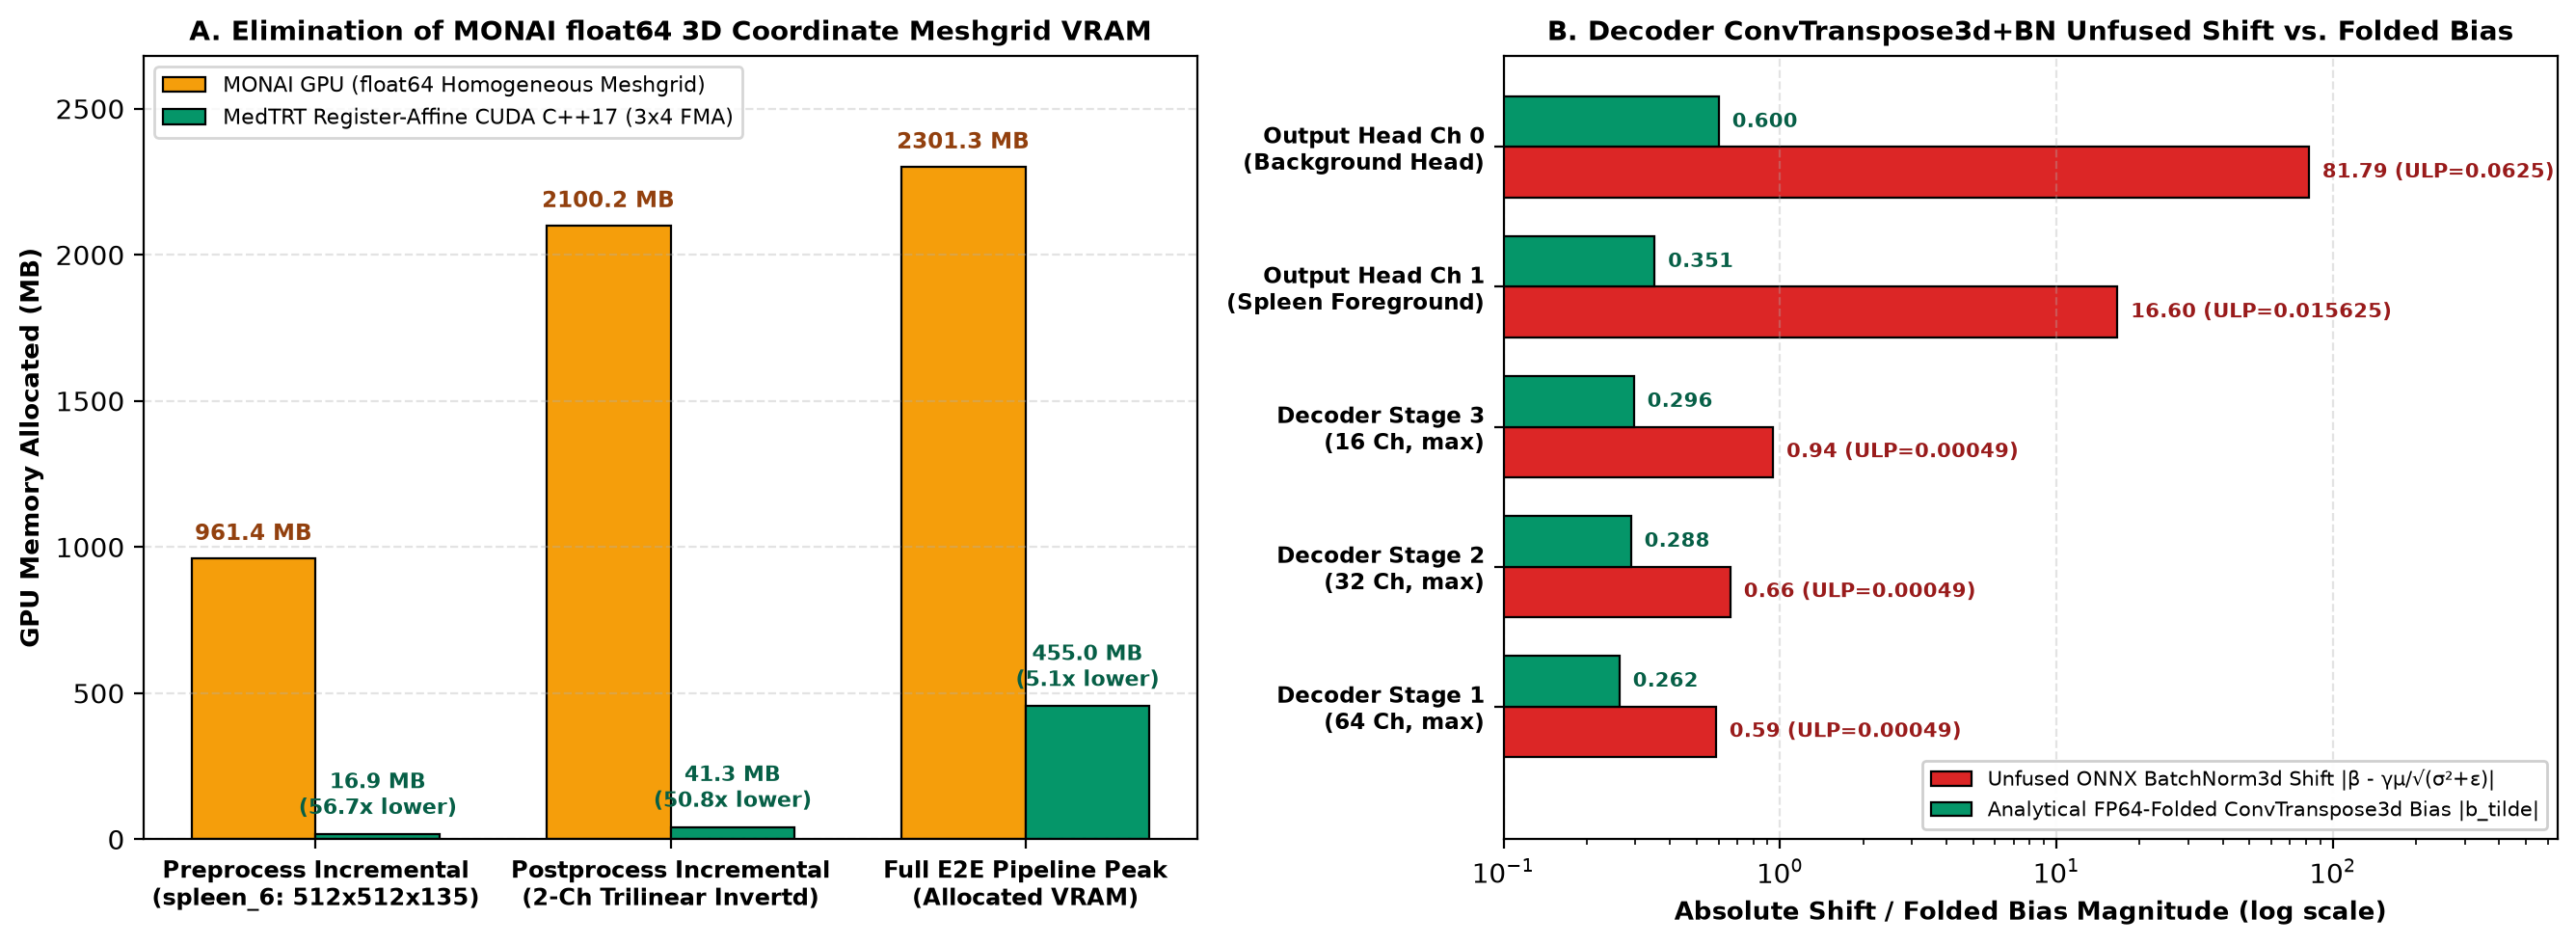
\includegraphics[width=0.90\textwidth]{figures/register_affine_mechanism.png}
    \caption{\textbf{Left (A):} Elimination of MONAI's \texttt{float64} 3D coordinate meshgrid VRAM via MedTRT register-affine CUDA C++17 kernels ($961.4 \to 16.9\text{ MB}$ in preprocessing; $2,100.2 \to 41.3\text{ MB}$ in postprocessing; $2,301.3 \to 455.0\text{ MB}$ peak E2E pipeline). \textbf{Right (B):} Magnitude comparison of unfused ONNX \texttt{BatchNorm3d} shifts vs.\ analytical FP64-folded \texttt{ConvTranspose3d} biases across all four decoder blocks.}
    \label{fig:reg_affine}
\end{figure*}

\section{Numerical Fidelity and Analytical FP64 BatchNorm Folding}
\label{sec:numerics}

\subsection{IEEE-754 Binary16 Quantization Spacing and Catastrophic Cancellation}
An IEEE-754 floating-point format with $p_{\text{sig}}$ significand bits ($p_{\text{sig}}=24$ for binary32 \texttt{FP32} with 23 explicit mantissa bits; $p_{\text{sig}}=11$ for binary16 \texttt{FP16} with 10 explicit mantissa bits) represents real magnitudes $x \in [2^E, 2^{E+1})$ with binade exponent $E = \lfloor \log_2 \lvert x \rvert \rfloor$ at discrete Unit in the Last Place ($\text{ULP}$, dimensionless step size) spacing:
\begin{equation}
    \text{ULP}(x) = 2^{E - (p_{\text{sig}} - 1)} = \begin{cases}
    2^{E - 23} & \text{in IEEE-754 FP32} \\
    2^{E - 10} & \text{in IEEE-754 FP16}
    \end{cases}
\end{equation}
On the interval $[64, 128)$ ($E = 6$), $\text{ULP}_{\text{FP32}} = 2^{-17} \approx 7.63 \times 10^{-6}$, whereas $\text{ULP}_{\text{FP16}} = 2^{6 - 10} = 2^{-4} = \mathbf{0.0625}$. When a pre-normalization activation $Y_0 \approx +57.6$ is quantized to the FP16 grid ($\text{ULP}_{[32,64)} = 0.03125$) and summed with an unfused affine shift of $-81.79$ ($\text{ULP}_{[64,128)} = 0.0625$) to yield a small logit near $+0.1$, subtracting nearly equal large numbers of opposite sign in 10-bit mantissa arithmetic destroys $6\text{--}7$ bits of significand precision via catastrophic cancellation.

\subsection{Asymmetric ONNX Constant Folding in 3D U-Net Decoders}
Compiling the standard PyTorch ONNX export (\texttt{opset 17}) into TensorRT 10.16 FP16 (\texttt{trt\_fp16\_unfolded}) produced a systematic volumetric dilation of $\mathbf{+1.6754 \pm 0.5531\textbf{ cm}^3}$ across $\mathbf{9/9}$ internal MSD validation scans ($p < 0.0001$) and $\mathbf{+1.5366 \pm 0.7680\textbf{ cm}^3}$ across $\mathbf{12/12}$ unseen external \texttt{FLARE22} scans ($\mathbf{+1.5961 \pm 0.6721\textbf{ cm}^3}$ across all $21/21$ pooled patients). Inspecting all 17 \texttt{BatchNorm3d} layers in \texttt{models/model.pt} revealed that PyTorch's ONNX constant folder fuses all \textbf{13 encoder \texttt{Conv3d+BatchNorm3d}} blocks, but \textbf{leaves all 4 decoder \texttt{ConvTranspose3d+BatchNorm3d} blocks unfused} (Table~\ref{tab:decoder_bn}). In the terminal 2-channel output head (\texttt{model.2.0.adn.N}), Channel 0 (background) carries convolution bias $b_0 = +57.295700$ against BatchNorm running mean $\mu_0 = +57.618198$ (variance $\sigma_0^2 = 2.132934$, weight $\gamma_0 = +2.100127$, bias $\beta_0 = +1.063365$, $\epsilon = 10^{-5}$), applying an unfused post-convolution shift:
\begin{equation}
\begin{aligned}
    \text{shift}_{\text{BN}, 0} &= \beta_0 - \frac{\gamma_0 \mu_0}{\sqrt{\sigma_0^2 + \epsilon}} \\
    &= 1.0634 - 57.6182 \times 1.4380 = \mathbf{-81.791538}
\end{aligned}
\end{equation}
Simultaneously, Channel 1 (spleen foreground) carries $b_1 = -18.385847$ and $\mu_1 = -18.462671$, applying an unfused shift of $\mathbf{+16.595694}$ ($\text{ULP}_{[16,32)} = 0.015625$). In FP16 execution, this asymmetric rounding depresses background logits by $-0.159$ and elevates foreground logits by $+0.116$, widening the decision margin $L_1 - L_0$ by $+0.275$ around splenic boundaries.

\subsection{Exact Analytical FP64 Weight Folding Derivation}
For a 3D transposed convolution (\texttt{nn.ConvTranspose3d}) with kernel tensor $W \in \mathbb{R}^{C_{\text{in}} \times C_{\text{out}} \times k_D \times k_H \times k_W}$ and bias $\mathbf{b} \in \mathbb{R}^{C_{\text{out}}}$ followed by \texttt{nn.BatchNorm3d} ($\boldsymbol{\gamma}, \boldsymbol{\beta}, \boldsymbol{\mu}, \boldsymbol{\sigma}^2, \epsilon = 10^{-5}$), let $s_c = \gamma_c / \sqrt{\sigma_c^2 + \epsilon}$. The pre-activation output $Z_c$ for output channel $c \in \{0, \dots, C_{\text{out}}-1\}$ given input feature map $X$ is:
\begin{equation}
\begin{aligned}
    Z_c &= s_c \left(\sum_{i=0}^{C_{\text{in}}-1} W_{i, c, :, :, :} *^\top X_i + b_c - \mu_c\right) + \beta_c \\
    &= \sum_{i=0}^{C_{\text{in}}-1} \underbrace{\left(W_{i, c, :, :, :} \cdot s_c\right)}_{\widetilde{W}_{i, c, :, :, :}} *^\top X_i + \underbrace{\big((b_c - \mu_c) s_c + \beta_c\big)}_{\widetilde{b}_c}
\end{aligned}
\label{eq:bn_fold}
\end{equation}
By promoting $W, \mathbf{b}, \boldsymbol{\gamma}, \boldsymbol{\beta}, \boldsymbol{\mu}, \boldsymbol{\sigma}^2$ to IEEE-754 \texttt{torch.float64} (53-bit significand) prior to ONNX export (\texttt{fold\_conv\_transpose\_batchnorm} in \texttt{src/medtrt/model.py}), evaluating $(b_0 - \mu_0) = -0.322498$ free of cancellation, casting $\widetilde{W}, \widetilde{\mathbf{b}}$ back to \texttt{float32}, and replacing \texttt{BatchNorm3d} with \texttt{nn.Identity()}, the $-81.79$ shift collapses into $\widetilde{b}_0 = +0.599613$ and $\widetilde{b}_1 = -0.351193$ (Table~\ref{tab:decoder_bn}). Strict FP32 outputs remain invariant ($\max \lvert \Delta\text{logit}\rvert = 1.43 \times 10^{-5}$; exported 53-node ONNX opset 17 graph $\max \lvert \Delta\text{logit}\rvert = 2.67 \times 10^{-5}$), while TensorRT FP16 mean absolute logit drift drops by $\mathbf{35.6\times}$ ($0.1377 \to 0.00387$) and internal MSD volumetric bias drops by over three orders of magnitude ($+1.6754\text{ cm}^3 \to +0.0010\text{ cm}^3$).

\begin{table*}[t]
\centering
\caption{Exact learned parameters of all four decoder \texttt{ConvTranspose3d+BatchNorm3d} blocks in \texttt{spleen\_ct\_segmentation} v0.6.1 (\texttt{models/model.pt}), demonstrating how analytical FP64 folding eliminates the $-81.79$ and $+16.60$ intermediate shifts in \texttt{model.2.0}.}
\label{tab:decoder_bn}
\resizebox{\textwidth}{!}{%
\begin{tabular}{lcccccc}
\toprule
\textbf{Decoder \texttt{ConvTranspose3d + BatchNorm3d} Block} & \textbf{$C_{\text{out}}$} & \textbf{Unfused Conv Bias $b_c$} & \textbf{BN Running Mean $\mu_c$} & \textbf{Scale $s_c = \frac{\gamma_c}{\sqrt{\sigma_c^2+\epsilon}}$} & \textbf{Unfused BN Shift $\beta_c - \mu_c s_c$} & \textbf{Folded Bias $\widetilde{b}_c = (b_c - \mu_c)s_c + \beta_c$} \\
\midrule
\texttt{model.1.submodule.1.submodule.1.submodule.2.0} (Stage 1) & $64$ & $[-0.196, +0.448]$ & $[-0.196, +0.448]$ & $\max 1.3193$ & $[-0.5858, +0.3007]$ & $\max 0.2621$ \\
\texttt{model.1.submodule.1.submodule.2.0} (Stage 2) & $32$ & $[-0.453, +0.395]$ & $[-0.453, +0.395]$ & $\max 1.6689$ & $[-0.5089, +0.6604]$ & $\max 0.2885$ \\
\texttt{model.1.submodule.2.0} (Stage 3) & $16$ & $[-0.569, +0.431]$ & $[-0.569, +0.431]$ & $\max 1.6712$ & $[-0.6951, +0.9425]$ & $\max 0.2956$ \\
\textbf{\texttt{model.2.0} (Channel 0: Background Head)} & $1$ (Ch0) & $\mathbf{+57.295700}$ & $\mathbf{+57.618198}$ & $\mathbf{+1.437999}$ & $\mathbf{-81.791538}$ ($\mathbf{-81.79}$) & $\mathbf{+0.599613}$ \\
\textbf{\texttt{model.2.0} (Channel 1: Spleen Foreground Head)} & $1$ (Ch1) & $\mathbf{-18.385847}$ & $\mathbf{-18.462671}$ & $\mathbf{+0.921735}$ & $\mathbf{+16.595694}$ ($\mathbf{+16.60}$) & $\mathbf{-0.351193}$ \\
\bottomrule
\end{tabular}%
}
\end{table*}

\section{Experimental Methodology, Secondary Engineering Problems, and Verification Infrastructure}
\label{sec:secondary_problems}

\subsection{Hardware Platform, Multi-Cohort Design, and Statistical Protocol}
All measurements were collected on an \textbf{NVIDIA GeForce RTX 5080 Laptop GPU} (Blackwell architecture, compute capability $12.0$ / \texttt{sm\_120}, $60$ SMs, $15.92\text{ GB}$ / $16,302\text{ MB}$ GDDR7, $90\text{ W}$ dynamic TGP, Windows 11 build \texttt{10.0.26300} in \texttt{WDDM} mode, NVIDIA Driver \texttt{591.44}, CUDA \texttt{12.8}, cuDNN \texttt{9.19.0}, TensorRT \texttt{10.16.1.11}, PyTorch \texttt{2.11.0+cu128}, MONAI \texttt{1.6.1}, Python \texttt{3.11.15}). TensorRT engines were built with dynamic batch profiles $B \in [1, 8]$ (optimization profile $B=2$, serialized size $13.70\text{ MB}$). Each benchmark executes 3 untimed warm-up volumes followed by repeated timed passes across the 9 held-out MSD scans ($90$ timed passes $= 10 \times 9$ on GPU-transform profiles; $18$ timed passes $= 2 \times 9$ on CPU-bound host profiles in \texttt{results/bench\_*.json}). Every stage is bracketed by hardware \texttt{torch.cuda.Event(enable\_timing=True)} pairs synchronized via \texttt{torch.cuda.synchronize()} and cross-checked against host \texttt{time.perf\_counter()} wall-clock timers (worst median gap $0.26\%$). NVTX annotations are embedded in \texttt{src/medtrt/timing.py} for optional Nsight Systems capture, though all reported latencies derive directly from CUDA Event and wall-clock telemetry.

We strictly separate pass-level timing stability from patient-level biological variance across two independent CT cohorts ($53$ total GPU-verified volumes):
\begin{itemize}
    \item \textbf{Cohort 1 (Internal MSD \texttt{Task09\_Spleen}, $N = 9$ validation / $41$ total CT scans):} Per upstream \texttt{configs/train.json} (\texttt{@images[-9:]}), the final 9 alphanumerically sorted scans (\texttt{spleen\_56} to \texttt{spleen\_9}) have zero overlap with the 32 gradient-update training scans. Because MSD test labels (\texttt{imagesTs}) are unannotated and upstream checkpoint selection used validation Dice on these 9 scans, absolute Dice ($0.9652$) serves as an internal baseline, whereas cross-backend deltas against strict IEEE FP32 (\texttt{pytorch\_fp32\_strict}) are exact.
    \item \textbf{Cohort 2 (External Unseen MICCAI \texttt{FLARE22}, $N = 12$ Multi-Center CT scans):} We evaluate 12 independent multi-center abdominal CT scans (\texttt{FLARE22\_Tr\_0001} to \texttt{0012}, $512 \times 512 \times 84\text{--}110$ voxels, spacing $0.64\text{--}0.86 \times 2.5\text{ mm}$, ground-truth spleen volumes $130.8\text{--}481.7\text{ cm}^3$) from Zenodo Record \texttt{7860267} \cite{ma2023flare}, streamed from cloud-mounted virtual storage (\texttt{results/external\_flare22\_validation.json}).
    \item \textbf{Formal Paired TOST Equivalence:} Because a non-significant two-sided $t$-test ($p = 0.885$) cannot prove numerical equivalence, we perform paired Two One-Sided Tests (TOST) \cite{schuirmann1987} at $\alpha = 0.05$ ($90\%$ confidence bounds) with margins $\Delta_V = \pm 0.10\text{ cm}^3$ ($< 0.04\%$ of mean spleen volume) and $\pm 0.50\text{ cm}^3$, plus $\Delta_{\text{Dice}} = \pm 0.0010$ and $\pm 0.0050$.
\end{itemize}

\subsection{Eight Secondary Engineering and Methodological Problems Resolved}
Beyond our three primary contributions, engineering MedTRT required resolving eight subtle systems and validation pitfalls:
\begin{enumerate}[label=\textbf{Problem \Alph*:},wide=0pt]
    \item \textbf{Deferred \texttt{mmap} Page-Fault Accounting \& Three-Regime I/O Decomposition:} Opening \texttt{.nii} files with \texttt{nibabel.load(..., mmap=True)} reduces \texttt{load} to $1.47\text{ ms}$ while raising \texttt{h2d} from $3.76\text{ ms}$ to $27.62\text{ ms}$ because OS virtual pages fault lazily during PCIe DMA transfer. We therefore report combined $\texttt{ingest} = \texttt{load} + \texttt{h2d}$ ($29.18\text{ ms}$ warm median) alongside standalone CPU \texttt{.nii.gz} decompression ($264.95\text{ ms}$) and cold unbuffered NVMe \texttt{.nii} reads ($23.83\text{ ms}$).
    \item \textbf{Staircase Aliasing in Nearest-Neighbor Discrete Inversion (\texttt{trt\_fp16\_nn}):} Discretizing at $1.5 \times 1.5 \times 2.0\text{ mm}$ prior to nearest-neighbor inversion (\texttt{trt\_fp16\_nn}) degrades Mean Dice by $\mathbf{-0.005004}$ ($0.965233 \to 0.960230$, violating the $0.005$ tolerance on $4/9$ scans). Kernel \#7 (\texttt{fused\_invert\_trilinear\_threshold\_u8}) preserves $100\%$ trilinear boundary smoothness in $2.62\text{ ms}$.
    \item \textbf{Paradoxical Masking of the $+1.68\text{ cm}^3$ FP16 Bug by Ground-Truth Capsule Under-Segmentation:} Because the pretrained 3D U-Net has higher precision ($0.9746$) than sensitivity ($0.9562$) and under-segments the outer 1-voxel splenic capsule relative to human annotations ($V_{\text{FP32}} - V_{\text{GT}} = -5.17 \pm 5.18\text{ cm}^3$), the buggy unfolded engine's $+1.68\text{ cm}^3$ dilation partially canceled against ground truth (yielding a deceptively lower MAE vs.\ GT of $4.24\text{ cm}^3$ vs.\ $5.17\text{ cm}^3$, Table~\ref{tab:metrics10}). Dual Bland--Altman and TOST testing against strict FP32 isolates numerical quantization drift from model anatomy error.
    \item \textbf{The ``All-Zeros / Blank Patch'' Unit-Test Trap:} Zero-filled synthetic tensors fail to excite decoder activations or trigger the $-81.79$ cancellation. In \texttt{tests/test\_engine\_accuracy.py}, we extract real anatomical patches centered on the spleen center of mass in \texttt{spleen\_6} (\texttt{patch.std() > 0.05}) and verify all $169$ sliding-window batches ($\text{probability\_mae} = 1.66 \times 10^{-6}$).
    \item \textbf{TensorRT 10.x Default-Stream Serialization \& Laptop GPU DVFS Clock Inflation (\texttt{P0} $\to$ \texttt{P4/P8}):} During the $\sim 2.7\text{ s}$ CPU resampling gap on host profiles, the laptop GPU downclocks to idle power states, inflating subsequent network execution by $\mathbf{1.13\times}$ after a $3\text{ s}$ idle interval ($290.7\text{ ms} \to 328.0\text{ ms}$ on TensorRT; $1,119.7\text{ ms} \to 1,267.6\text{ ms}$ on TF32). We bind TensorRT \texttt{execute\_async\_v3} to a dedicated non-default CUDA stream (\texttt{self.exec\_stream}) synchronized via hardware events.
    \item \textbf{Confounded Speedup Claims \& Non-Additivity of Marginal Stage Medians ($\sum_k \text{median}(T_k) \neq \text{median}(\sum_k T_k)$):} Across heterogeneous slice counts ($Z \in [31, 135]$), marginal stage medians do not sum to the median of end-to-end pass totals ($29.2 + 1.3 + 49.0 + 6.1 + 2.6 = 88.2\text{ ms}$ vs.\ $96.3\text{ ms}$ E2E in \texttt{trt\_fp16\_cuda}). We report all six stages explicitly and strictly separate matched-window speedups ($\omega=0.5, B=4$: $30.67\times$ cohort / $33.14\times$ paired mean) from fast-window speedups ($\omega=0.25, B=8$: $42.86\times$ cohort / $46.64\times$ paired median).
    \item \textbf{False-Positive / False-Negative Volumetric Cancellation at the Splenic Hilum (\texttt{spleen\_62} vs.\ \texttt{spleen\_56}):} In \texttt{spleen\_62} (Dice $0.9611$, $\text{HD}_{95} = 2.44\text{ mm}$), $4,566$ FP voxels and $4,821$ FN voxels along hilar vessels cancel to $-0.58\text{ cm}^3$ net volume error, whereas in \texttt{spleen\_56} ($7.0\text{ mm}$ slices, Dice $0.9361$), $40\%$ of error voxels concentrate in the single polar slice at each dome. Volumetric agreement must therefore be paired with surface distance metrics ($\text{HD}_{95}$, $\text{ASSD}$).
    \item \textbf{Process-Wide PyTorch TF32 Flag Bleed Across Cached Streamlit Predictors:} Because \texttt{torch.backends.cudnn.allow\_tf32} is a process-global flag, caching multiple predictors in Streamlit caused TF32 state bleed until we enforced \texttt{apply\_precision(profile)} per inference call in \texttt{app/workstation.py} and verified isolation in \texttt{tests/test\_workstation.py}.
\end{enumerate}

\subsection{Software Architecture, 3D Tri-Planar Workstation, and Automated Claim Verification}
To make MedTRT self-auditing and directly usable by researchers, the repository integrates three software layers:
\begin{enumerate}
    \item \textbf{Fingerprinted Core Package (\texttt{src/medtrt/}):} Eight frozen measurement modules (\texttt{bench.py}, \texttt{data.py}, \texttt{evaluate.py}, \texttt{infer.py}, \texttt{model.py}, \texttt{profiles.py}, \texttt{timing.py}, \texttt{trt\_runner.py}) are hashed via normalized SHA-256 (\texttt{code\_fingerprint = e9d4f060aaf1b130}) alongside the compiled engine (\texttt{engine\_fingerprint = 28d585aaed46e401}) and stamped into all 29 JSON/CSV telemetry artifacts in \texttt{results/}.
    \item \textbf{Interactive 3D Tri-Planar Workstation \& Telemetry Dashboard (\texttt{app/viewer.py}, \texttt{app/workstation.py}, \texttt{app/dashboard/}):} A 10-page interactive analytics dashboard and radiological review workstation providing synchronized axial, coronal, and sagittal slice navigation, decoupled screen-only HU windowing presets (Soft Tissue $W=400, L=40$; Bone $W=1800, L=400$; Lung $W=1500, L=-600$), 1-pixel contour overlays, live side-by-side backend comparison with signed-boundary-distance FP32-vs-FP16 voxel difference heatmaps, and automatic suppression of ground-truth metrics on unlabeled uploads.
    \item \textbf{Offline Claim Verifier \& CI Suite (\texttt{src/medtrt/verify\_claims.py}, \texttt{tests/}):} Running \texttt{python -m medtrt.verify\_claims} executes 14 deterministic checks (verifying single code/engine provenance, recomputing medians and Bland--Altman/TOST bounds from raw passes, checking zero training-split leakage, confirming \texttt{README.md} byte-identity with \texttt{report.py}, and scanning for local path leaks or unsupported clinical language), complemented by 66 \texttt{pytest} tests and GitHub Actions CI (\texttt{.github/workflows/ci.yml}).
\end{enumerate}

\section{Quantitative Results}
\label{sec:results}

\subsection{End-to-End Pipeline Latency, Ablation, and 53-Volume Scaling}
Tables~\ref{tab:master}--\ref{tab:scaling53} and Figures~\ref{fig:stage_ablation} and \ref{fig:mem_pareto} summarize end-to-end performance across all 13 profiles and 53 CT volumes:
\begin{enumerate}
    \item \textbf{Controlled Like-for-Like Speedup (\texttt{trt\_fp16\_cuda}, $\omega=0.5, B=4$):} Keeping sliding-window overlap ($0.5$), batch size ($4$), and total patch evaluations ($665$ windows across the 9 MSD scans) identical to \texttt{pytorch\_fp32} ($2,952.0\text{ ms}$ median E2E) and \texttt{pytorch\_fp32\_strict} ($3,049.8\text{ ms}$), \texttt{trt\_fp16\_cuda} achieves $\mathbf{96.3\textbf{ ms}}$ cohort median latency (IQR $58.9\text{ ms}$, per-case range $47.6\text{--}162.4\text{ ms}$, slowest pass $232.6\text{ ms}$). This yields a $\mathbf{30.67\times}$ cohort median speedup ($\mathbf{31.68\times}$ vs.\ strict FP32) and a paired patient-level mean speedup of $\mathbf{33.14\times}$ ($95\%$ CI $[27.61\times, 38.67\times]$, median $31.00\times$, range $26.19\times\text{--}49.79\times$, Table~\ref{tab:percase}). Relative to MONAI's GPU pipeline (\texttt{trt\_fp16\_gpu}, $215.5\text{ ms}$), custom register-affine CUDA kernels accelerate E2E inference by $2.24\times$ while slashing peak allocated VRAM by $\mathbf{5.06\times}$ ($2,301\text{ MB} \to \mathbf{455\textbf{ MB}}$).
    \item \textbf{Fast-Window Operating Point (\texttt{trt\_\allowbreak fp16\_\allowbreak optimized}, $\omega=0.25, B=8$) \& 12-Point Pareto Sweep:} Across a 12-configuration sweep over $\omega \in \{0.25, 0.50, 0.75\} \times B \in \{1, 2, 4, 8\}$ (\texttt{results/\allowbreak sweep.csv}, Figure~\ref{fig:mem_pareto} Top Right), $(\omega=0.50, B=4)$ ($66.5\text{ ms}$ SW, Dice $0.965229$) and $(\omega=0.25, B=4)$ ($30.4\text{ ms}$ SW, Dice $0.964778$) form the measured Pareto frontier. Selecting $(\omega=0.25, B=8)$ for \texttt{trt\_\allowbreak fp16\_\allowbreak optimized} reduces patch evaluations from $665$ to $369$ ($1.80\times$ fewer patches) and achieves $\mathbf{68.9\textbf{ ms}}$ median E2E latency (IQR $50.5\text{ ms}$, slowest pass $122.6\text{ ms}$ across all 90 passes, $\mathbf{42.86\times}$ cohort speedup, $\mathbf{44.87\times}$ paired mean speedup, $\mathbf{46.64\times}$ paired median speedup) at $522\text{ MB}$ peak VRAM with a $-0.000455$ Mean Dice trade-off.
    \item \textbf{Multi-Cohort Scaling Across All 53 CT Volumes (Table~\ref{tab:scaling53}):} Across all 41 MSD patient scans ($8.13\text{M}\text{--}44.04\text{M}$ voxels, $31\text{--}168$ slices), \texttt{trt\_fp16\_optimized} maintains $\mathbf{87.44\textbf{ ms}}$ median E2E latency ($1.59\text{ ms}$ CUDA preprocess, $33.83\text{ ms}$ network, $3.28\text{ ms}$ CUDA postprocess, $450.6\text{ MB}$ median / $630.8\text{ MB}$ max VRAM). Across the 12 unseen external \texttt{FLARE22} volumes streamed over virtualized cloud-drive storage, \texttt{trt\_fp16\_cuda} achieves a $\mathbf{21.52\times}$ paired speedup ($5,422.9\text{ ms} \to 252.6\text{ ms}$, where $175.4\text{ ms}$ is cloud-drive I/O and only $2.75\text{ ms}$ and $3.38\text{ ms}$ are CUDA preprocessing and postprocessing; $220.6\text{ ms}$ / $24.29\times$ on \texttt{optimized}) while cutting peak VRAM by $\mathbf{4.56\times}$ ($1,885\text{ MB} \to 414\text{ MB}$).
\end{enumerate}

\begin{figure*}[t]
    \centering
    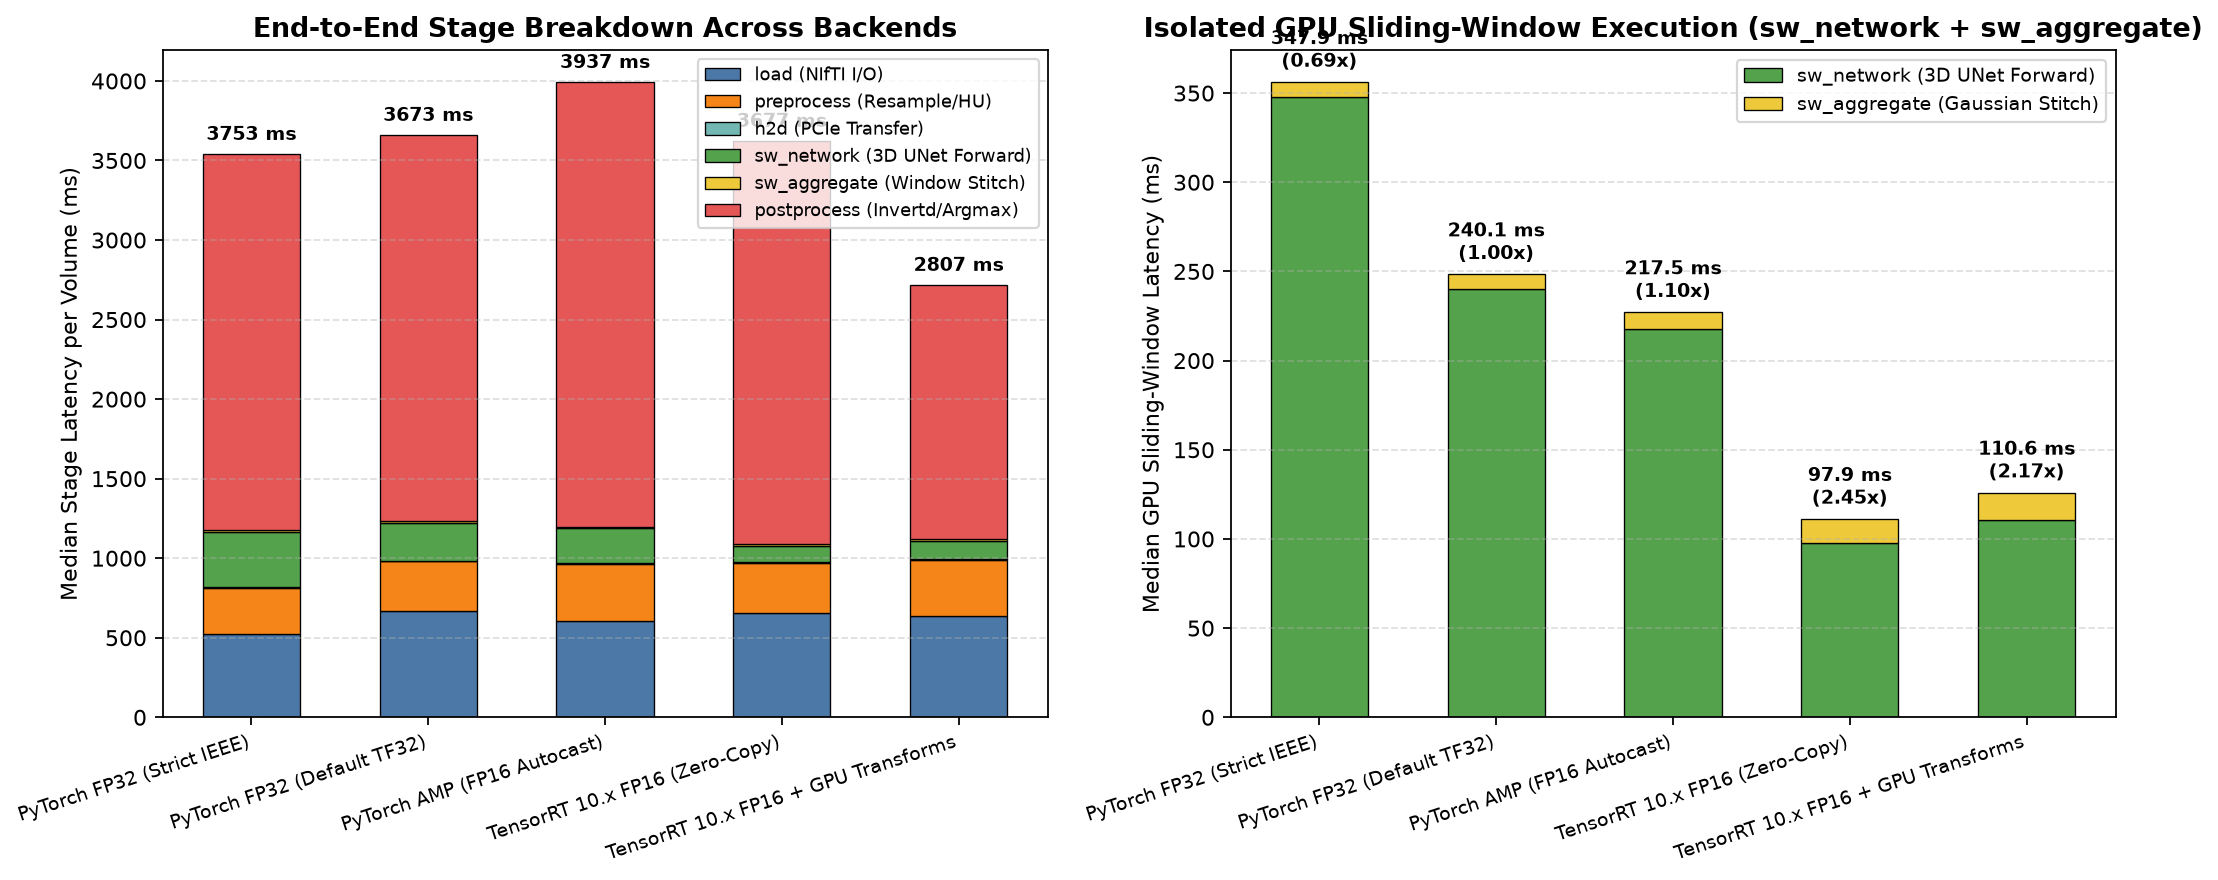
\includegraphics[width=0.46\textwidth]{figures/stage_breakdown.png}\hfill
    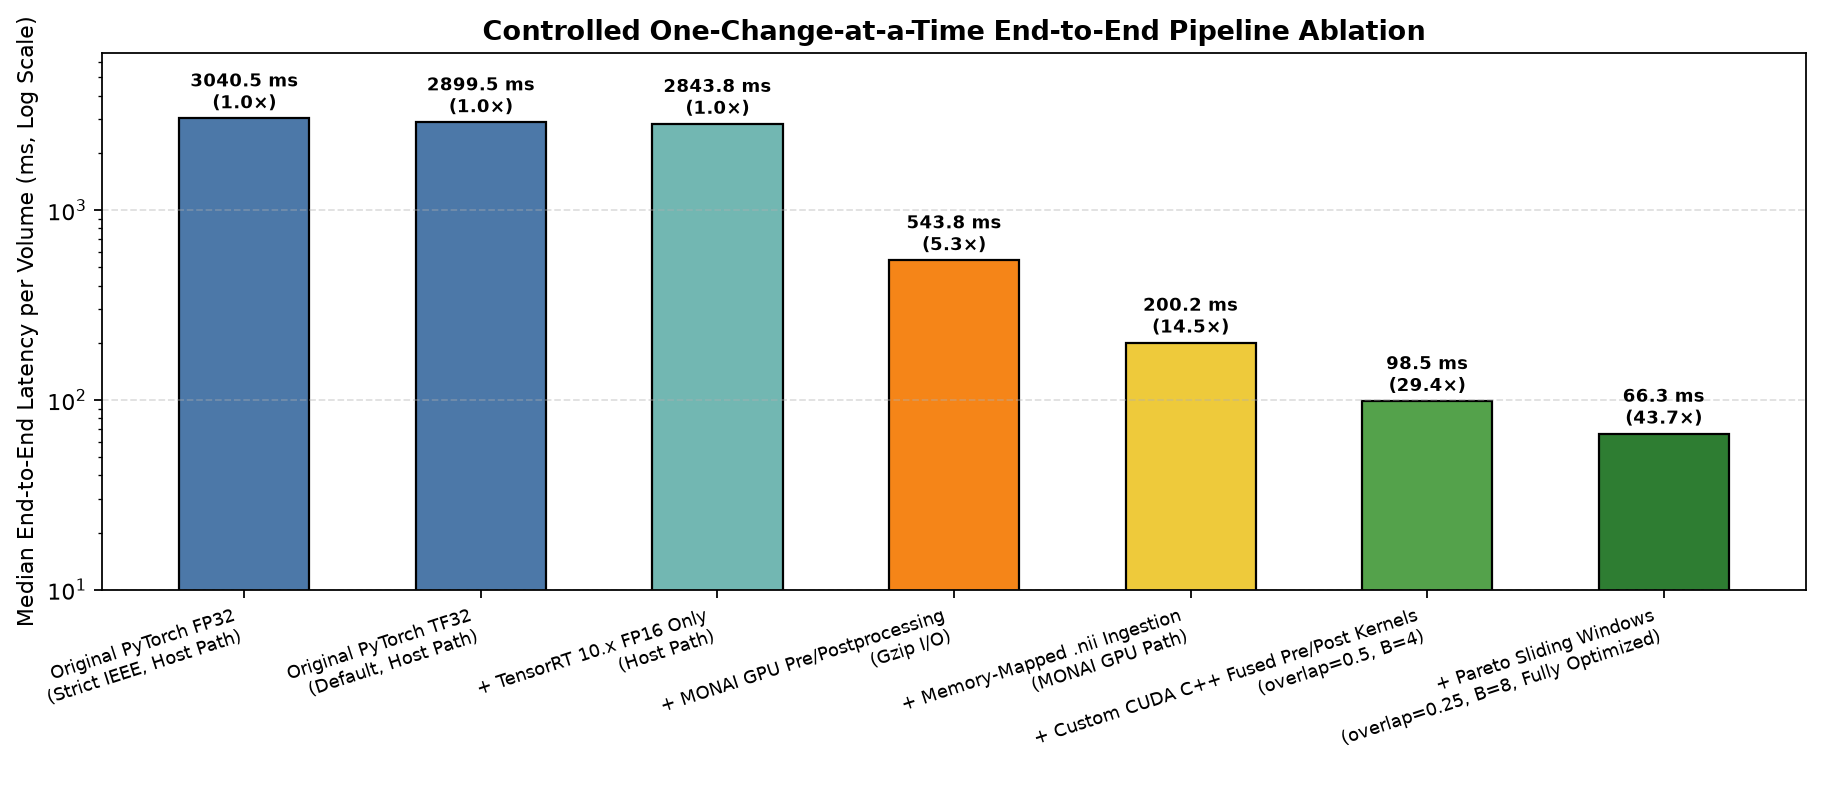
\includegraphics[width=0.46\textwidth]{figures/ablation_waterfall.png}\\[3pt]
    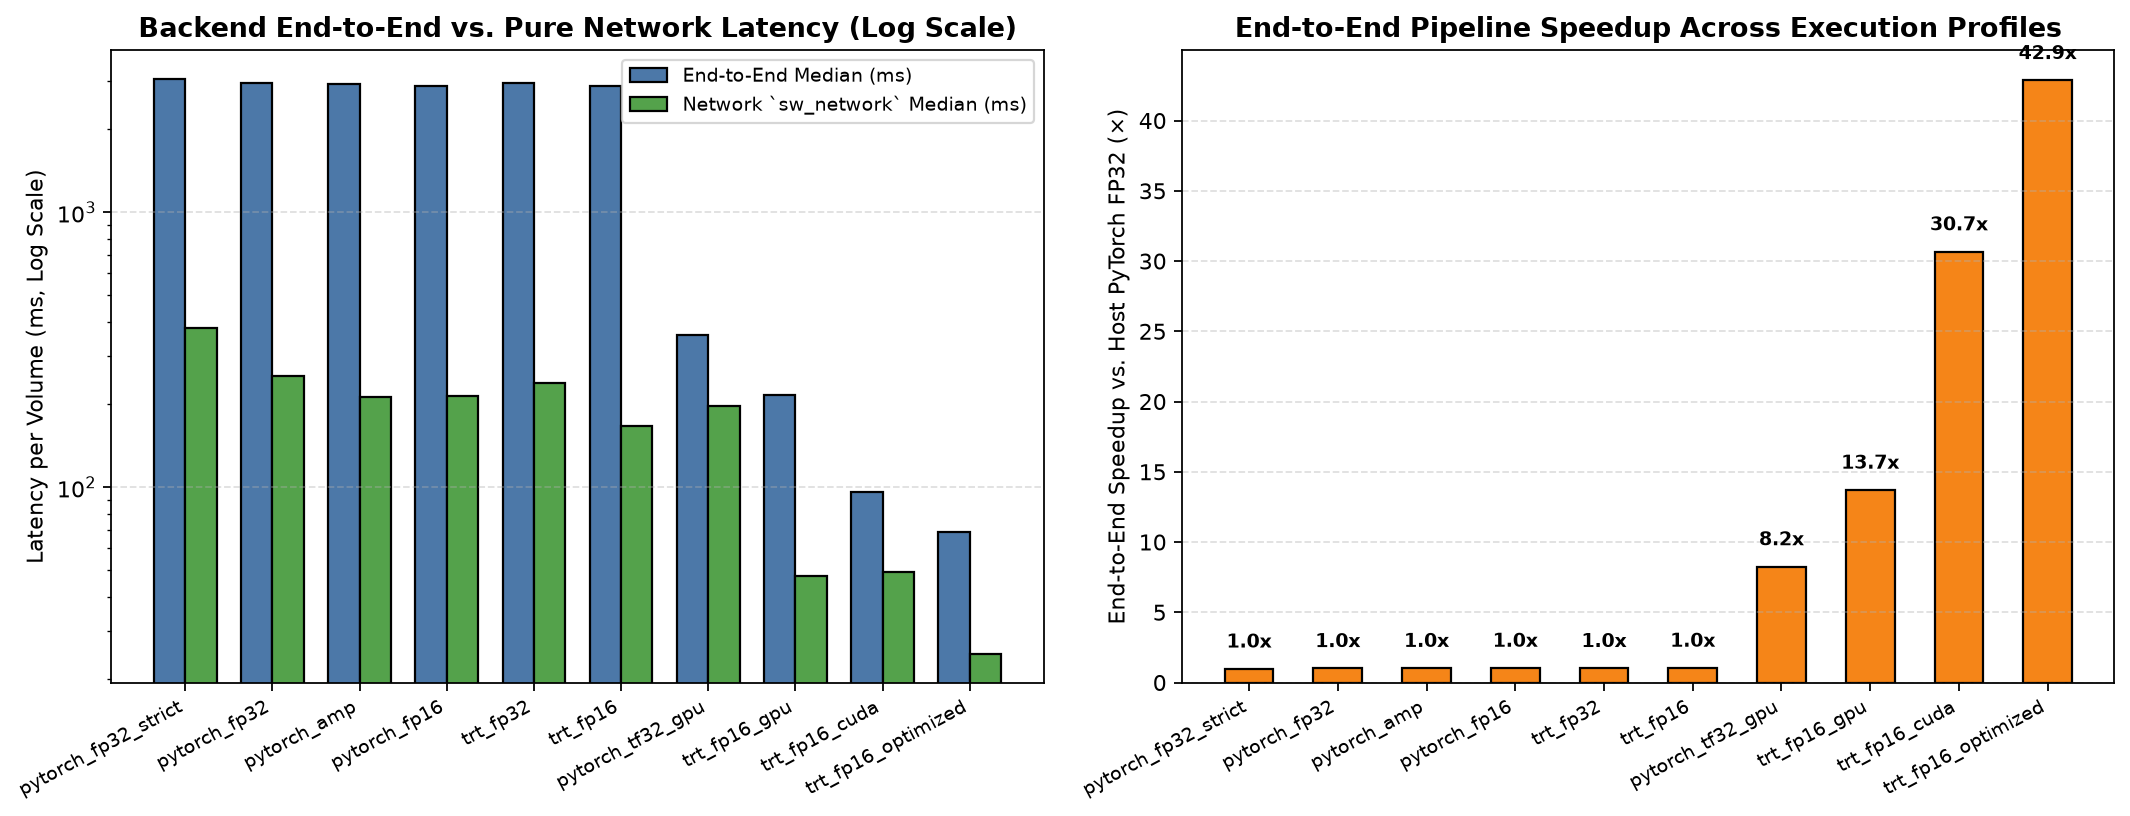
\includegraphics[width=0.46\textwidth]{figures/backend_latency_speedup.png}\hfill
    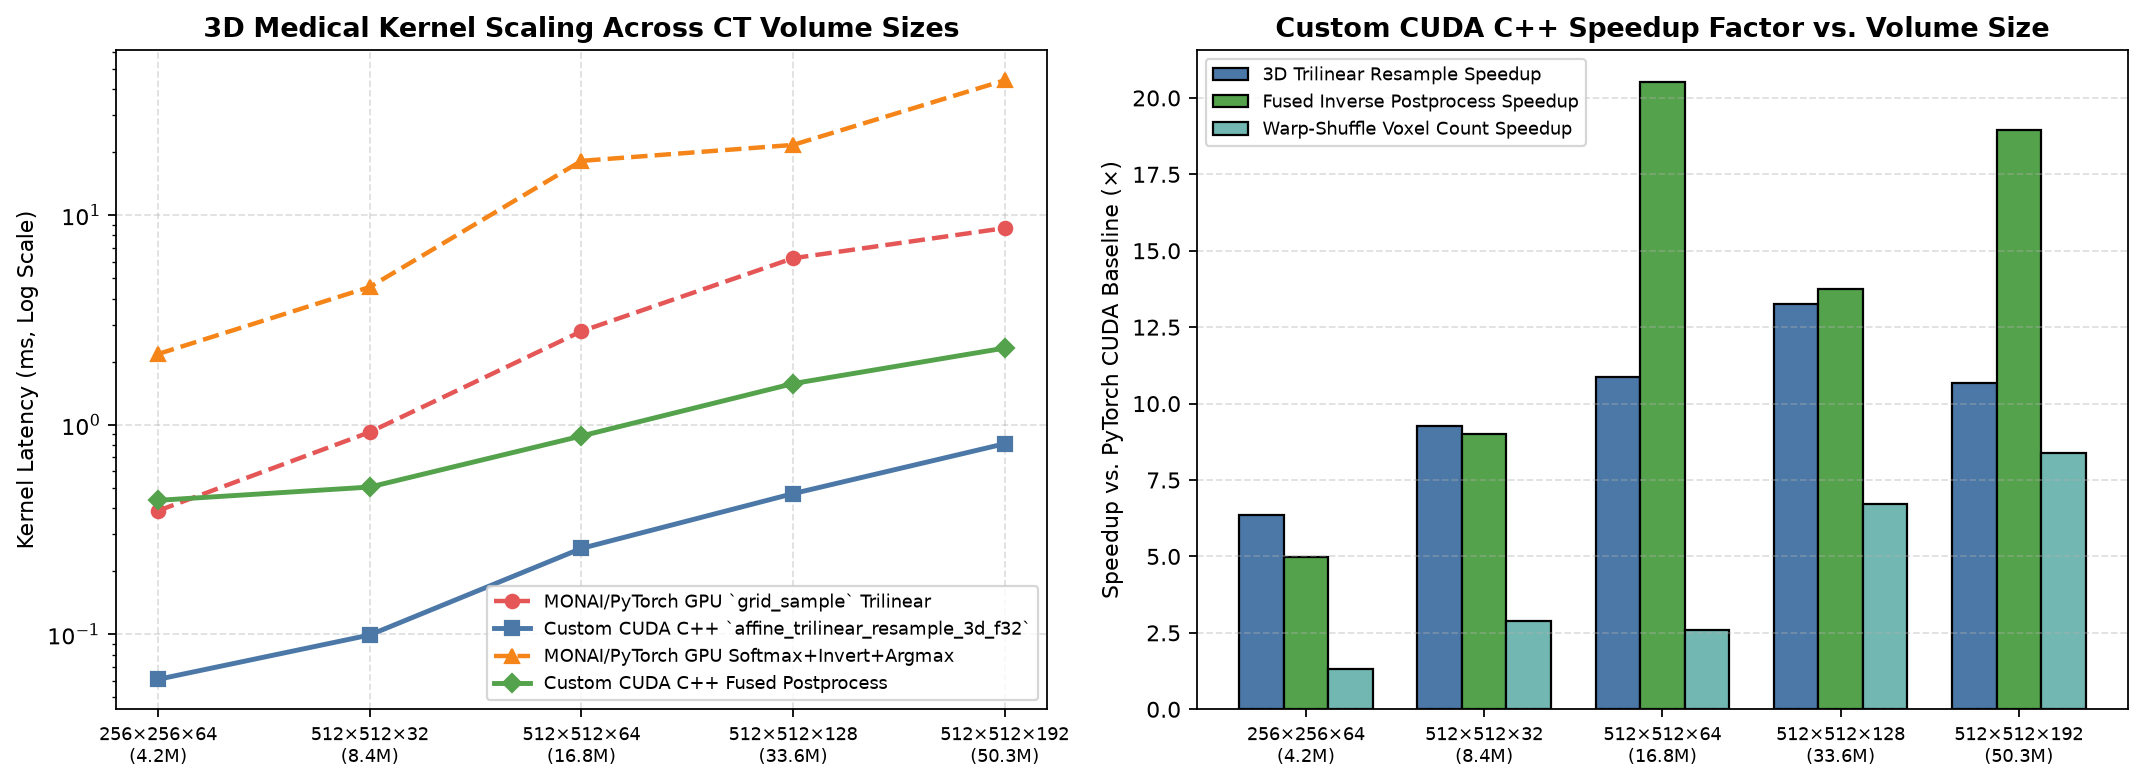
\includegraphics[width=0.46\textwidth]{figures/cuda_kernel_scaling.png}
    \caption{\textbf{Top Left:} Six-stage median latency decomposition across host and GPU execution paths on Cohort 1 ($N=9$ MSD scans). \textbf{Top Right:} Controlled one-factor-at-a-time ablation waterfall isolating the latency impact of each systems optimization. \textbf{Bottom Left:} End-to-end latency and speedup across all 13 benchmarked profiles. \textbf{Bottom Right:} Custom CUDA C++17 kernel latency and VRAM scaling across CT volume sizes vs.\ PyTorch and MONAI GPU transforms.}
    \label{fig:stage_ablation}
\end{figure*}

\begin{table*}[t]
\centering
\caption{Complete 13-profile benchmark and volumetric validation matrix on Cohort 1 (MSD \texttt{Task09\_Spleen}, $N = 9$ held-out patients on RTX 5080 Laptop GPU). All six pipeline stages are reported explicitly ($\texttt{Ingest} = \texttt{load} + \texttt{h2d}$). GPU-path profiles execute 90 timed passes ($10 \times 9$) and CPU-bound host profiles execute 18 timed passes ($2 \times 9$) in \texttt{results/bench\_*.json} (90-pass host reference runs at $3,341.1\text{ ms}$ E2E are archived in \texttt{docs/CLAIM\_VERIFICATION\_REPORT.md}).}
\label{tab:master}
\resizebox{\textwidth}{!}{%
\begin{tabular}{lcccccccccccc}
\toprule
\textbf{Profile} & \textbf{Path / I/O} & \textbf{Win / $B$} & \textbf{Ingest} & \textbf{Pre} & \textbf{Net} & \textbf{Agg} & \textbf{Post} & \textbf{E2E Med [IQR] (ms)} & \textbf{Cohort / Paired Speedup} & \textbf{Peak VRAM} & \textbf{Mean Dice $\pm$ SD} & \textbf{Vol Bias vs.\ FP32 Ref} \\
\midrule
\texttt{pytorch\_fp32\_strict} & CPU / gzip & $0.5/4$ & $367.4$ & $288.0$ & $379.9$ & $8.4$ & $2024.8$ & $3049.8$ [$3235.4$] & $0.97\times$ / $0.94\times$ & $490\text{ MB}$ & $0.965233 \pm 0.0117$ & Reference ($0.000\text{ cm}^3$) \\
\texttt{pytorch\_fp32} & CPU / gzip & $0.5/4$ & $424.7$ & $286.4$ & $254.6$ & $8.0$ & $1990.4$ & $2,952.0$ [$2970.8$] & $1.00\times$ / $1.00\times$ & $487\text{ MB}$ & $0.965228 \pm 0.0117$ & $+0.005 \pm 0.004\text{ cm}^3$ \\
\texttt{pytorch\_tf32} & CPU / gzip & $0.5/4$ & $424.7$ & $286.4$ & $254.6$ & $8.0$ & $1990.4$ & $2,952.0$ [$2970.8$] & $1.00\times$ / $1.00\times$ & $487\text{ MB}$ & $0.965228 \pm 0.0117$ & $+0.005 \pm 0.004\text{ cm}^3$ \\
\texttt{pytorch\_amp} & CPU / gzip & $0.5/4$ & $419.7$ & $271.7$ & $213.4$ & $9.1$ & $2013.6$ & $2916.1$ [$2954.5$] & $1.01\times$ / $0.99\times$ & $457\text{ MB}$ & $0.965217 \pm 0.0118$ & $+0.003 \pm 0.011\text{ cm}^3$ \\
\texttt{pytorch\_fp16} & CPU / gzip & $0.5/4$ & $340.1$ & $281.6$ & $213.9$ & $9.6$ & $1993.2$ & $2885.5$ [$2822.2$] & $1.02\times$ / $1.01\times$ & $458\text{ MB}$ & $0.965231 \pm 0.0118$ & $+0.025 \pm 0.015\text{ cm}^3$ \\
\texttt{trt\_fp32} & CPU / gzip & $0.5/4$ & $373.0$ & $276.7$ & $239.8$ & $8.9$ & $1981.5$ & $2940.0$ [$3003.2$] & $1.00\times$ / $1.00\times$ & $368\text{ MB}$ & $0.965233 \pm 0.0117$ & $+0.000 \pm 0.000\text{ cm}^3$ \\
\texttt{trt\_fp16\_unfolded} (Bug) & CPU / gzip & $0.5/4$ & $406.5$ & $273.2$ & $176.7$ & $36.7$ & $1994.5$ & $2866.4$ [$2909.5$] & $1.03\times$ / $1.03\times$ & $359\text{ MB}$ & $0.965722 \pm 0.0120$ & $\mathbf{+1.675 \pm 0.553\textbf{ cm}^3}$ \\
\texttt{trt\_fp16} (Folded) & CPU / gzip & $0.5/4$ & $385.1$ & $266.8$ & $167.1$ & $36.0$ & $1993.9$ & $2880.3$ [$2893.9$] & $1.02\times$ / $1.04\times$ & $359\text{ MB}$ & $0.965226 \pm 0.0117$ & $+0.003 \pm 0.022\text{ cm}^3$ \\
\texttt{pytorch\_tf32\_gpu} & GPU / mmap & $0.5/4$ & $38.8$ & $54.4$ & $197.0$ & $6.5$ & $62.2$ & $357.9$ [$244.6$] & $8.25\times$ / $8.76\times$ & $2,307\text{ MB}$ & $0.965227 \pm 0.0117$ & $+0.003 \pm 0.005\text{ cm}^3$ \\
\texttt{trt\_fp16\_gpu} & GPU / mmap & $0.5/4$ & $38.9$ & $43.9$ & $47.6$ & $6.5$ & $71.1$ & $215.5$ [$173.7$] & $13.70\times$ / $14.67\times$ & $2,301\text{ MB}$ & $0.965228 \pm 0.0117$ & $+0.001 \pm 0.017\text{ cm}^3$ \\
\textbf{\texttt{trt\_fp16\_cuda}} & \textbf{CUDA / mmap} & $\mathbf{0.5/4}$ & $\mathbf{29.2}$ & $\mathbf{1.3}$ & $\mathbf{49.0}$ & $\mathbf{6.1}$ & $\mathbf{2.6}$ & $\mathbf{96.3}$ [$\mathbf{58.9}$] & $\mathbf{30.67\times}$ / $\mathbf{33.14\times}$ & $\mathbf{455\textbf{ MB}}$ & $\mathbf{0.965229 \pm 0.0117}$ & $\mathbf{+0.001 \pm 0.019\textbf{ cm}^3}$ \\
\textbf{\texttt{trt\_fp16\_optimized}} & \textbf{CUDA / mmap} & $\mathbf{0.25/8}$ & $\mathbf{29.1}$ & $\mathbf{1.3}$ & $\mathbf{24.8}$ & $\mathbf{4.5}$ & $\mathbf{2.8}$ & $\mathbf{68.9}$ [$\mathbf{50.5}$] & $\mathbf{42.86\times}$ / $\mathbf{44.87\times}$ & $\mathbf{522\textbf{ MB}}$ & $\mathbf{0.964778 \pm 0.0135}$ & $+0.120 \pm 1.182\text{ cm}^3$ \\
\texttt{trt\_fp16\_nn} & GPU / mmap & $0.25/8$ & $38.1$ & $41.7$ & $20.8$ & $4.1$ & $69.3$ & $178.4$ [$141.3$] & $16.55\times$ / $16.89\times$ & $2,149\text{ MB}$ & $0.960230 \pm 0.0139$ & $+0.481 \pm 1.073\text{ cm}^3$ \\
\bottomrule
\end{tabular}%
}
\end{table*}

\begin{table}[t]
\centering
\caption{Controlled 9-rung one-factor-at-a-time ablation ladder (\texttt{results/ablation.json}) plus custom CUDA operating points (\texttt{results/bench\_*.json}) on Cohort 1 ($N = 9$ scans).}
\label{tab:ablation}
\resizebox{\columnwidth}{!}{%
\begin{tabular}{lccccc}
\toprule
\textbf{Configuration (Single Factor Changed)} & \textbf{E2E Med} & \textbf{Max} & \textbf{Speedup} & \textbf{Net} & \textbf{Mean Dice} \\
\midrule
1. Host path, PyTorch TF32 (\texttt{gzip + CPU}) & $2992.5$ & $6339.3$ & $1.00\times$ & $239.3$ & $0.965228$ \\
2. Host path, TensorRT FP16 only & $2923.0$ & $6015.0$ & $1.02\times$ & $170.3$ & $0.965226$ \\
3. MONAI GPU transforms, \texttt{gzip} read, TF32 & $706.9$ & $1404.3$ & $4.23\times$ & $201.1$ & $0.965228$ \\
4. MONAI GPU transforms, \texttt{gzip} read, TRT & $564.3$ & $1252.9$ & $5.30\times$ & $47.2$ & $0.965228$ \\
5. MONAI GPU transforms, \texttt{.nii} read, TF32 & $363.3$ & $686.1$ & $8.24\times$ & $195.9$ & $0.965228$ \\
6. MONAI GPU transforms, \texttt{.nii} read, TRT & $274.8$ & $472.5$ & $10.89\times$ & $54.0$ & $0.965228$ \\
7. Fast windows ($\omega=0.25, B=8$), MONAI GPU, TF32 & $320.6$ & $540.4$ & $9.33\times$ & $111.9$ & $0.964771$ \\
8. Fast windows ($\omega=0.25, B=8$), MONAI GPU, TRT & $218.5$ & $374.2$ & $13.70\times$ & $23.5$ & $0.964767$ \\
9. Fast windows, MONAI GPU, nearest inverse & $219.0$ & $361.6$ & $13.66\times$ & $24.1$ & $0.960230$ \\
\midrule
\textbf{+ Custom CUDA Kernels L4L (\texttt{trt\_fp16\_cuda})} & $\mathbf{96.3}$ & $\mathbf{232.6}$ & $\mathbf{31.07\times}$ & $\mathbf{49.0}$ & $\mathbf{0.965229}$ \\
\textbf{+ Custom CUDA Kernels Fast (\texttt{optimized})} & $\mathbf{68.9}$ & $\mathbf{122.6}$ & $\mathbf{43.43\times}$ & $\mathbf{24.8}$ & $\mathbf{0.964778}$ \\
\bottomrule
\end{tabular}%
}
\end{table}

\begin{table*}[t]
\centering
\caption{Multi-cohort GPU scaling across all $\mathbf{53}$ \textbf{abdominal 3D CT volumes} ($41$ MSD volumes on local NVMe $+ 12$ unseen external MICCAI \texttt{FLARE22} volumes streamed over virtualized cloud-drive storage).}
\label{tab:scaling53}
\resizebox{\textwidth}{!}{%
\begin{tabular}{lcccccccccc}
\toprule
\textbf{Cohort Subset \& Execution Profile} & \textbf{Vols ($N$)} & \textbf{Voxel Range ($512 \times 512 \times Z$)} & \textbf{Patch Windows} & \textbf{\texttt{ingest} Med} & \textbf{\texttt{preprocess} Med} & \textbf{\texttt{sw\_network} Med} & \textbf{\texttt{postprocess} Med} & \textbf{E2E Median [IQR] (ms)} & \textbf{E2E Min--Max (ms)} & \textbf{Peak VRAM Med / Max} \\
\midrule
\textbf{MSD Full Cohort (\texttt{trt\_fp16\_optimized})} & $\mathbf{41}$ & $8.13\text{M}\text{--}44.04\text{M}$ ($Z \in [31, 168]$) & $16\text{--}75$ (med $48$) & $41.32\text{ ms}$ & $\mathbf{1.59\textbf{ ms}}$ & $33.83\text{ ms}$ & $\mathbf{3.28\textbf{ ms}}$ & $\mathbf{87.44}$ [$\mathbf{43.55}$] & $37.61\text{--}139.84$ & $450.6$ / $\mathbf{630.8\textbf{ MB}}$ \\
\textbf{MSD Training Split (\texttt{trt\_fp16\_optimized})} & $32$ & $10.49\text{M}\text{--}44.04\text{M}$ ($Z \in [40, 168]$) & $16\text{--}75$ (med $48$) & $41.70\text{ ms}$ & $1.50\text{ ms}$ & $33.84\text{ ms}$ & $3.34\text{ ms}$ & $87.77$ [$40.52$] & $48.82\text{--}131.82$ & $478.8$ / $630.8\text{ MB}$ \\
\textbf{MSD Validation Split (\texttt{optimized}, 90-pass)} & $\mathbf{9}$ & $8.13\text{M}\text{--}35.39\text{M}$ ($Z \in [31, 135]$) & $18\text{--}64$ (med $32$) & $29.14\text{ ms}$ & $\mathbf{1.27\textbf{ ms}}$ & $\mathbf{24.77\textbf{ ms}}$ & $\mathbf{2.84\textbf{ ms}}$ & $\mathbf{68.88}$ [$\mathbf{50.48}$] & $33.92\text{--}122.59$ & $394.3$ / $\mathbf{522.1\textbf{ MB}}$ \\
\textbf{External \texttt{FLARE22} (\texttt{trt\_fp16\_cuda})} & $\mathbf{12}$ & $22.02\text{M}\text{--}28.84\text{M}$ ($Z \in [84, 110]$) & $32\text{--}72$ (med $50$) & $175.4\text{ ms}$ (Cloud) & $\mathbf{2.75\textbf{ ms}}$ & $64.5\text{ ms}$ & $\mathbf{3.38\textbf{ ms}}$ & $\mathbf{252.6}$ [$\mathbf{27.2}$] & $221.5\text{--}276.2$ & $373.0$ / $\mathbf{414.0\textbf{ MB}}$ \\
\textbf{External \texttt{FLARE22} (\texttt{trt\_fp16\_optimized})} & $\mathbf{12}$ & $22.02\text{M}\text{--}28.84\text{M}$ ($Z \in [84, 110]$) & $18\text{--}32$ (med $32$) & $175.0\text{ ms}$ (Cloud) & $\mathbf{2.73\textbf{ ms}}$ & $36.1\text{ ms}$ & $\mathbf{3.37\textbf{ ms}}$ & $\mathbf{220.6}$ [$\mathbf{33.6}$] & $197.9\text{--}247.3$ & $373.0$ / $\mathbf{414.0\textbf{ MB}}$ \\
\bottomrule
\end{tabular}%
}
\end{table*}

\subsection{Ten-Metric Geometric Validation, External Generalization, and TOST Equivalence}
Tables~\ref{tab:metrics10}--\ref{tab:tost} and Figures~\ref{fig:mem_pareto} and \ref{fig:tradeoff_ba} detail segmentation accuracy and cross-backend numerical equivalence across all $N = 21$ validation patients:
\begin{itemize}
    \item \textbf{Ten-Metric Overlap, Surface, and Volumetric Fidelity (Table~\ref{tab:metrics10}):} Across all 10 evaluation metrics in \texttt{results/eval\_*.csv}, \texttt{trt\_fp16\_cuda} matches strict IEEE FP32 (\texttt{pytorch\_fp32\_strict}) to four-to-six significant digits: Mean Dice $0.965229$ vs.\ $0.965233$, IoU $0.933011$ vs.\ $0.933019$, Sensitivity $0.956189$ vs.\ $0.956191$, Precision $0.974553$ vs.\ $0.974558$, Specificity $0.999853$ vs.\ $0.999853$, Volumetric Similarity $0.990461$ vs.\ $0.990460$, $\text{HD}_{95} = 2.18\text{ mm}$ vs.\ $2.18\text{ mm}$, and $\text{ASSD} = 0.3894\text{ mm}$ vs.\ $0.3892\text{ mm}$. Across all $9$ internal MSD validation cases, Dice shows no significant correlation with slice thickness (Spearman $\rho = -0.13, p = 0.74$) or ground-truth volume ($\rho = +0.23, p = 0.55$); the coarsest scan (\texttt{spleen\_8}, $7.5\text{ mm}$) ranks first in Dice ($0.9734$).
    \item \textbf{Formal Paired TOST Equivalence Across $N = 21$ Patients (Table~\ref{tab:tost}):} Unfolded TensorRT FP16 (\texttt{trt\_fp16\_unfolded}) fails equivalence on every cohort ($+1.6754\text{ cm}^3$ on MSD, $+1.5366\text{ cm}^3$ on \texttt{FLARE22}, $+1.5961\text{ cm}^3$ pooled; $p_{\text{TOST}} \ge 0.9997$, flipping $586.9$ voxels or $0.644\%$ per spleen on MSD). Analytical FP64 weight folding (\texttt{trt\_fp16\_cuda}) satisfies paired TOST equivalence at $\alpha = 0.05$ within the strict $\Delta_V = \pm 0.10\text{ cm}^3$ bound on internal MSD ($+0.0010 \pm 0.0194\text{ cm}^3$, $90\%$ CI $[-0.0110, +0.0130]\text{ cm}^3$, $p_{\text{TOST}} < 10^{-6}$), external \texttt{FLARE22} ($-0.0110 \pm 0.0315\text{ cm}^3$, $90\%$ CI $[-0.0274, +0.0053]\text{ cm}^3$, $p_{\text{TOST}} < 10^{-6}$), and pooled $N = 21$ cohorts ($-0.0059 \pm 0.0271\text{ cm}^3$, $90\%$ CI $[-0.0161, +0.0043]\text{ cm}^3$, $p_{\text{TOST}} < 10^{-6}$), flipping an average of only $8.8$ boundary voxels ($0.0093\%$) on MSD and $22.6$ voxels ($0.0208\%$) on \texttt{FLARE22}.
    \item \textbf{External Multi-Center Pathology Generalization (Table~\ref{tab:percase}):} On the 12 unseen \texttt{FLARE22} scans, the frozen model achieves $0.9360 \pm 0.0493$ Mean Dice ($0.9554\text{--}0.9665$ across 9 typical scans; $0.8286\text{--}0.9043$ on 3 severe splenomegaly or boundary-variant cases with $V_{\text{GT}}$ up to $481.7\text{ cm}^3$), confirming that FP64-folded FP16 numerical equivalence holds even on out-of-distribution multi-center anatomy.
\end{itemize}

\begin{table*}[t]
\centering
\caption{Ten-metric geometric overlap, boundary distance, and physical volumetry summary (\texttt{results/eval\_*.csv}, Mean $\pm$ SD across Cohort 1 MSD $N=9$, ground-truth spleen volume $V_{\text{GT}} = 286.73 \pm 130.35\text{ cm}^3$).}
\label{tab:metrics10}
\resizebox{\textwidth}{!}{%
\begin{tabular}{lcccccccccc}
\toprule
\textbf{Execution Profile} & \textbf{3D Dice} & \textbf{IoU (Jaccard)} & \textbf{Sensitivity} & \textbf{Precision} & \textbf{Specificity} & \textbf{Vol.\ Similarity} & \textbf{$\text{HD}_{95}$ (mm)} & \textbf{ASSD (mm)} & \textbf{$V_{\text{pred}}$ ($\text{cm}^3$)} & \textbf{MAE vs.\ GT / Bias vs.\ FP32} \\
\midrule
\texttt{pytorch\_fp32\_strict} (Ref) & $0.965233 \pm 0.0117$ & $0.933019 \pm 0.0215$ & $0.956191 \pm 0.0158$ & $0.974558 \pm 0.0119$ & $0.999853$ & $0.990460 \pm 0.0079$ & $2.18 \pm 0.99$ & $0.389 \pm 0.119$ & $281.56 \pm 128.29$ & $5.17\text{ cm}^3$ / $0.0000\text{ cm}^3$ \\
\texttt{trt\_fp16\_unfolded} (Bug) & $0.965722 \pm 0.0120$ & $0.933942 \pm 0.0219$ & $0.959719 \pm 0.0155$ & $0.971909 \pm 0.0127$ & $0.999838$ & $0.992356 \pm 0.0064$ & $2.45 \pm 1.80$ & $0.391 \pm 0.121$ & $283.24 \pm 128.83$ & $4.24\text{ cm}^3$ / $\mathbf{+1.6754\textbf{ cm}^3}$ \\
\textbf{\texttt{trt\_fp16\_cuda} (Folded L4L)} & $\mathbf{0.965229 \pm 0.0117}$ & $\mathbf{0.933011 \pm 0.0215}$ & $\mathbf{0.956189 \pm 0.0158}$ & $\mathbf{0.974553 \pm 0.0119}$ & $\mathbf{0.999853}$ & $\mathbf{0.990461 \pm 0.0080}$ & $\mathbf{2.18 \pm 0.99}$ & $\mathbf{0.389 \pm 0.119}$ & $\mathbf{281.56 \pm 128.29}$ & $5.17\text{ cm}^3$ / $\mathbf{+0.0010\textbf{ cm}^3}$ \\
\textbf{\texttt{trt\_fp16\_optimized} (Fast)} & $\mathbf{0.964778 \pm 0.0135}$ & $\mathbf{0.932236 \pm 0.0246}$ & $\mathbf{0.955821 \pm 0.0166}$ & $\mathbf{0.973997 \pm 0.0136}$ & $\mathbf{0.999853}$ & $\mathbf{0.990435 \pm 0.0071}$ & $\mathbf{2.35 \pm 1.81}$ & $\mathbf{0.417 \pm 0.133}$ & $\mathbf{281.68 \pm 128.52}$ & $5.10\text{ cm}^3$ / $+0.1196\text{ cm}^3$ \\
\texttt{trt\_fp16\_nn} (Nearest Inv) & $0.960230 \pm 0.0139$ & $0.923798 \pm 0.0250$ & $0.951877 \pm 0.0169$ & $0.968824 \pm 0.0140$ & $0.999822$ & $0.991007 \pm 0.0072$ & $2.44 \pm 1.80$ & $0.467 \pm 0.148$ & $282.04 \pm 128.54$ & $4.75\text{ cm}^3$ / $+0.4814\text{ cm}^3$ \\
\bottomrule
\end{tabular}%
}
\end{table*}

\begin{figure*}[t]
    \centering
    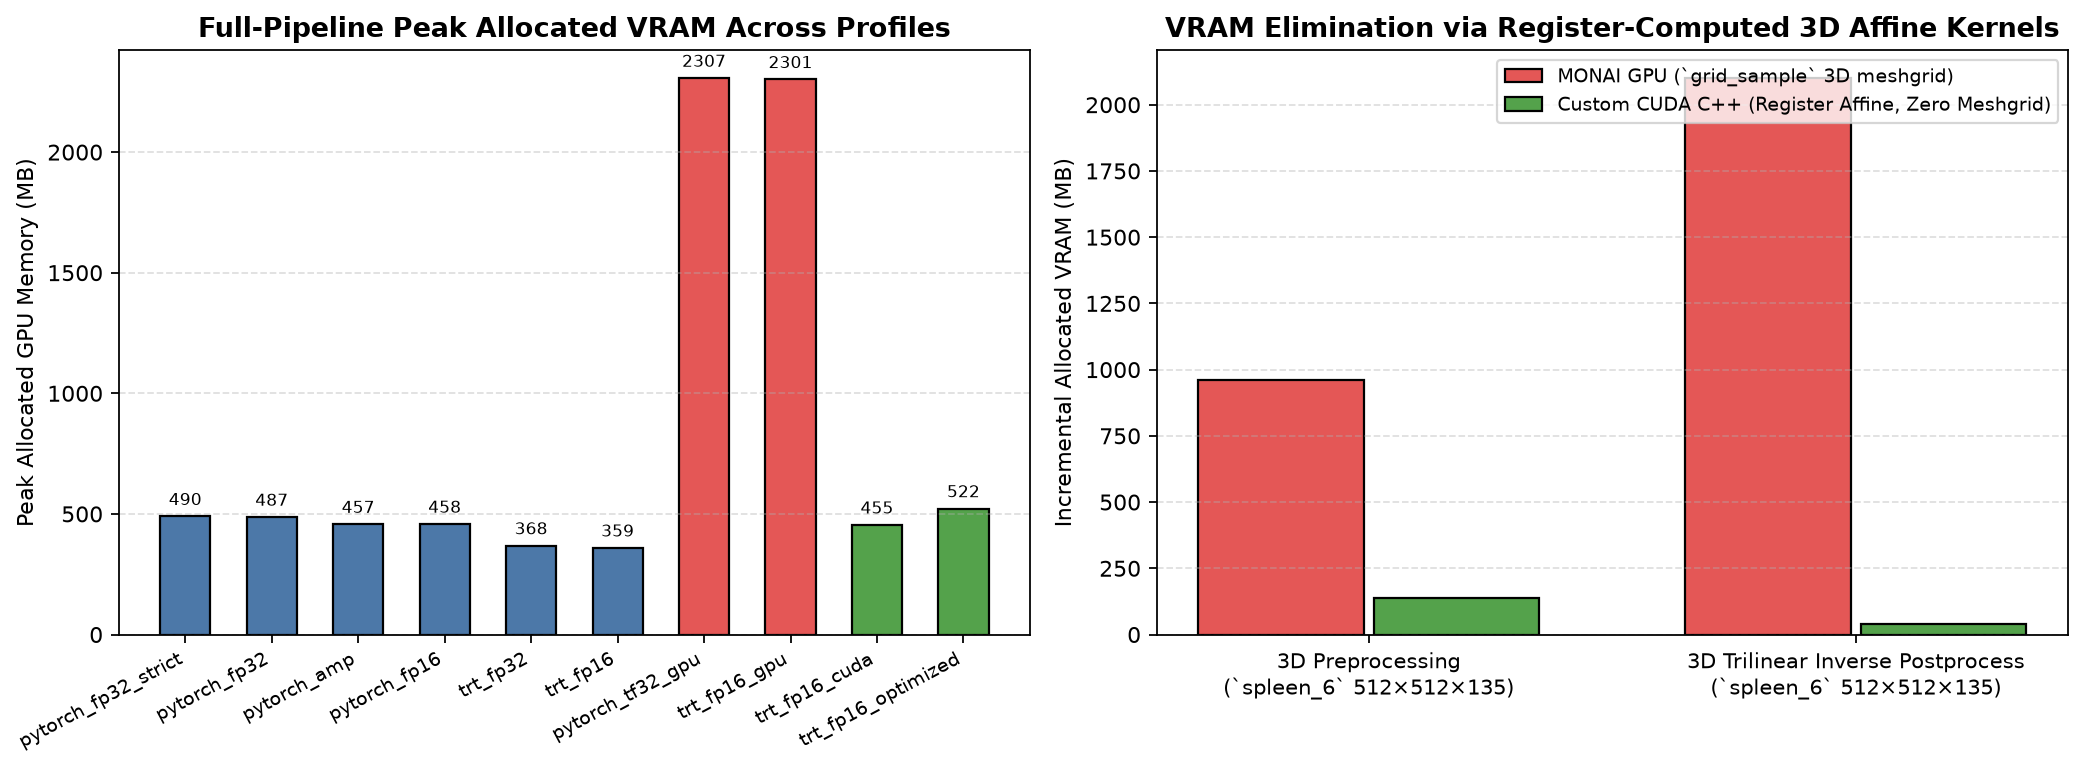
\includegraphics[width=0.45\textwidth]{figures/gpu_memory_comparison.png}\hfill
    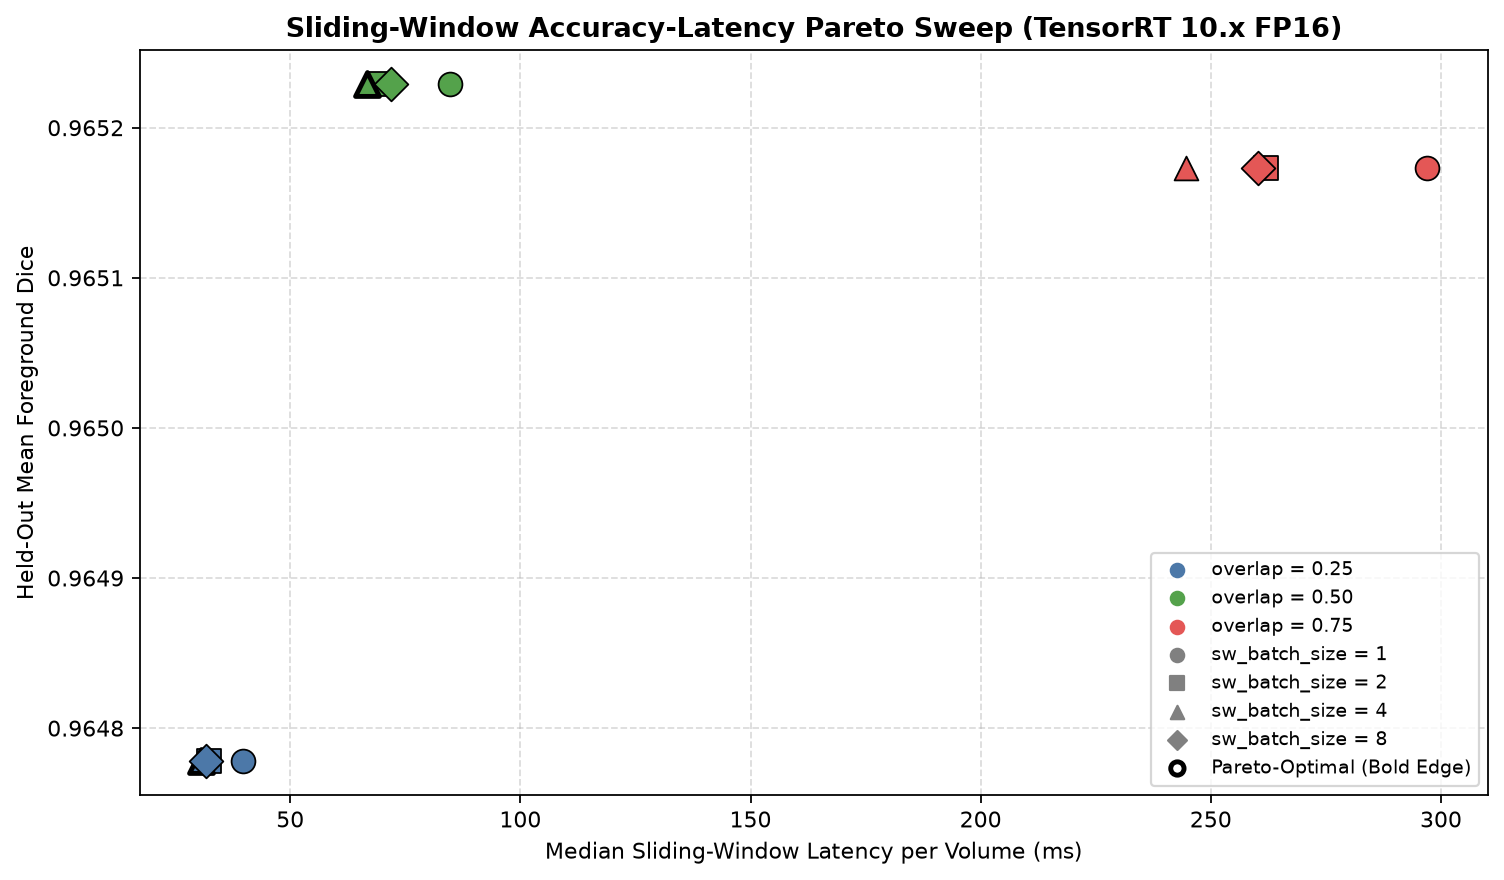
\includegraphics[width=0.45\textwidth]{figures/pareto_sweep.png}\\[3pt]
    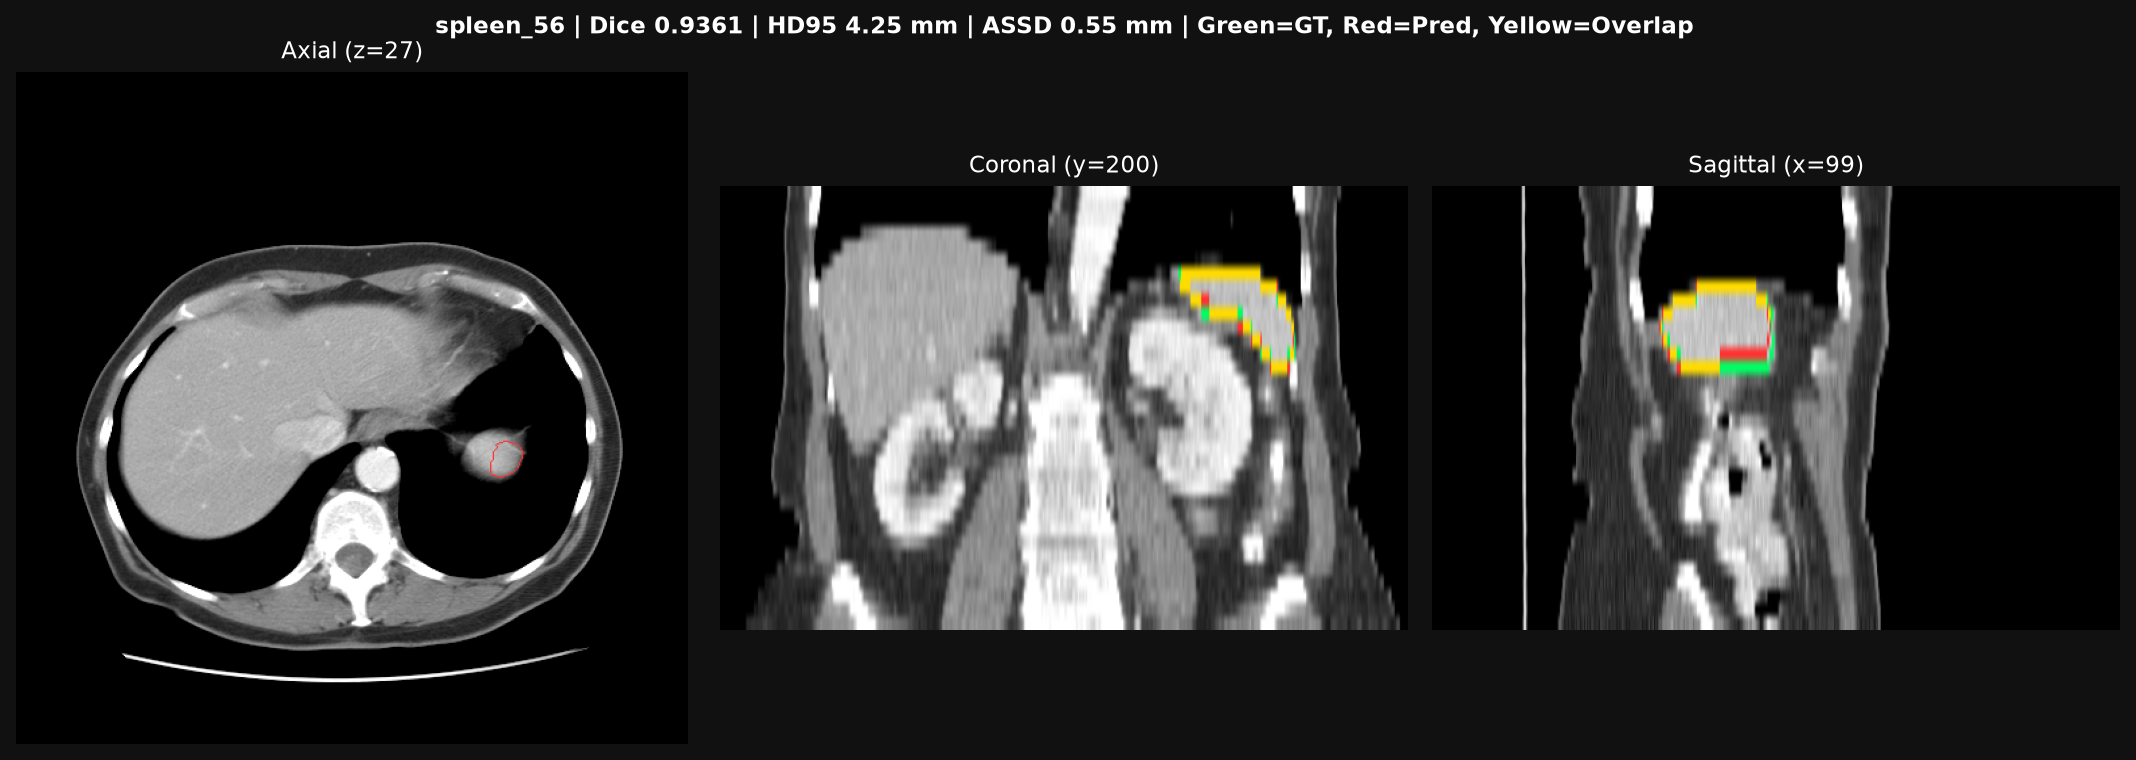
\includegraphics[width=0.44\textwidth]{figures/failure_case_1.png}\hfill
    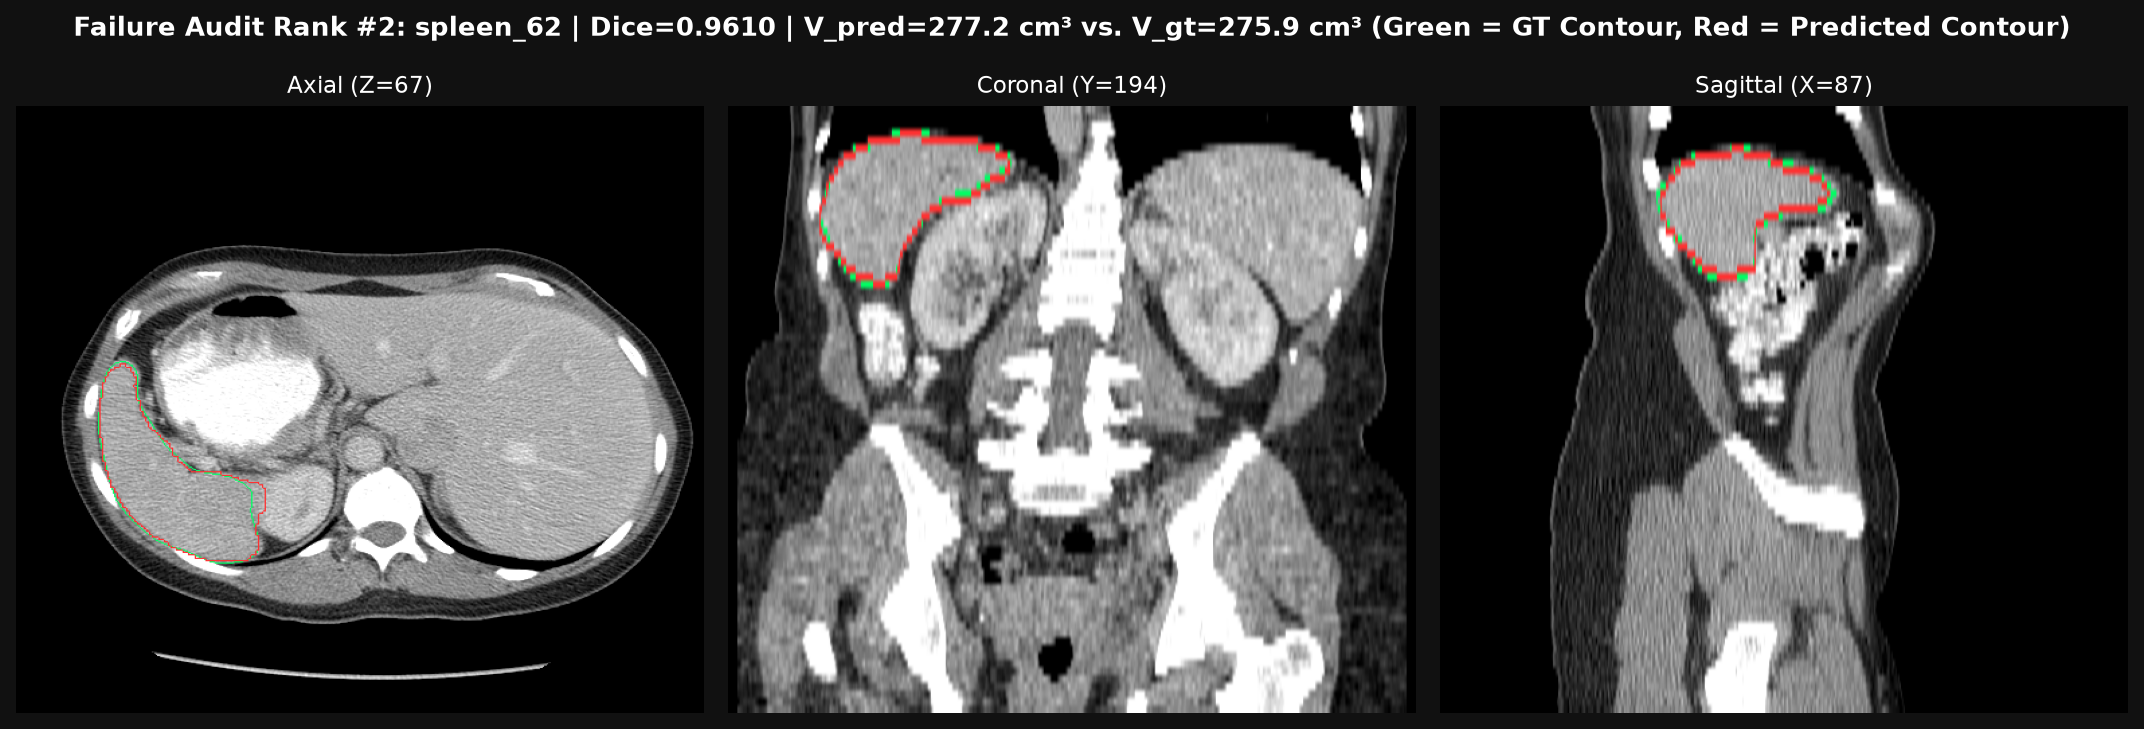
\includegraphics[width=0.44\textwidth]{figures/failure_case_2.png}
    \caption{\textbf{Top Left:} Peak GPU VRAM allocation ($2,301\text{ MB}$ MONAI \texttt{float64} meshgrids vs.\ $455\text{ MB}$ MedTRT register-affine CUDA). \textbf{Top Right:} 12-configuration sliding-window Pareto sweep across overlap $\omega \in \{0.25, 0.50, 0.75\}$ and batch size $B \in \{1, 2, 4, 8\}$. \textbf{Bottom Left:} Boundary analysis of \texttt{spleen\_56} (Dice $0.9361$, $7.0\text{ mm}$ slices) showing $40\%$ of error voxels at polar domes. \textbf{Bottom Right:} Boundary analysis of \texttt{spleen\_62} (Dice $0.9611$) showing FP/FN volumetric cancellation ($-0.58\text{ cm}^3$ net error) at the splenic hilum.}
    \label{fig:mem_pareto}
\end{figure*}

\begin{figure*}[t]
    \centering
    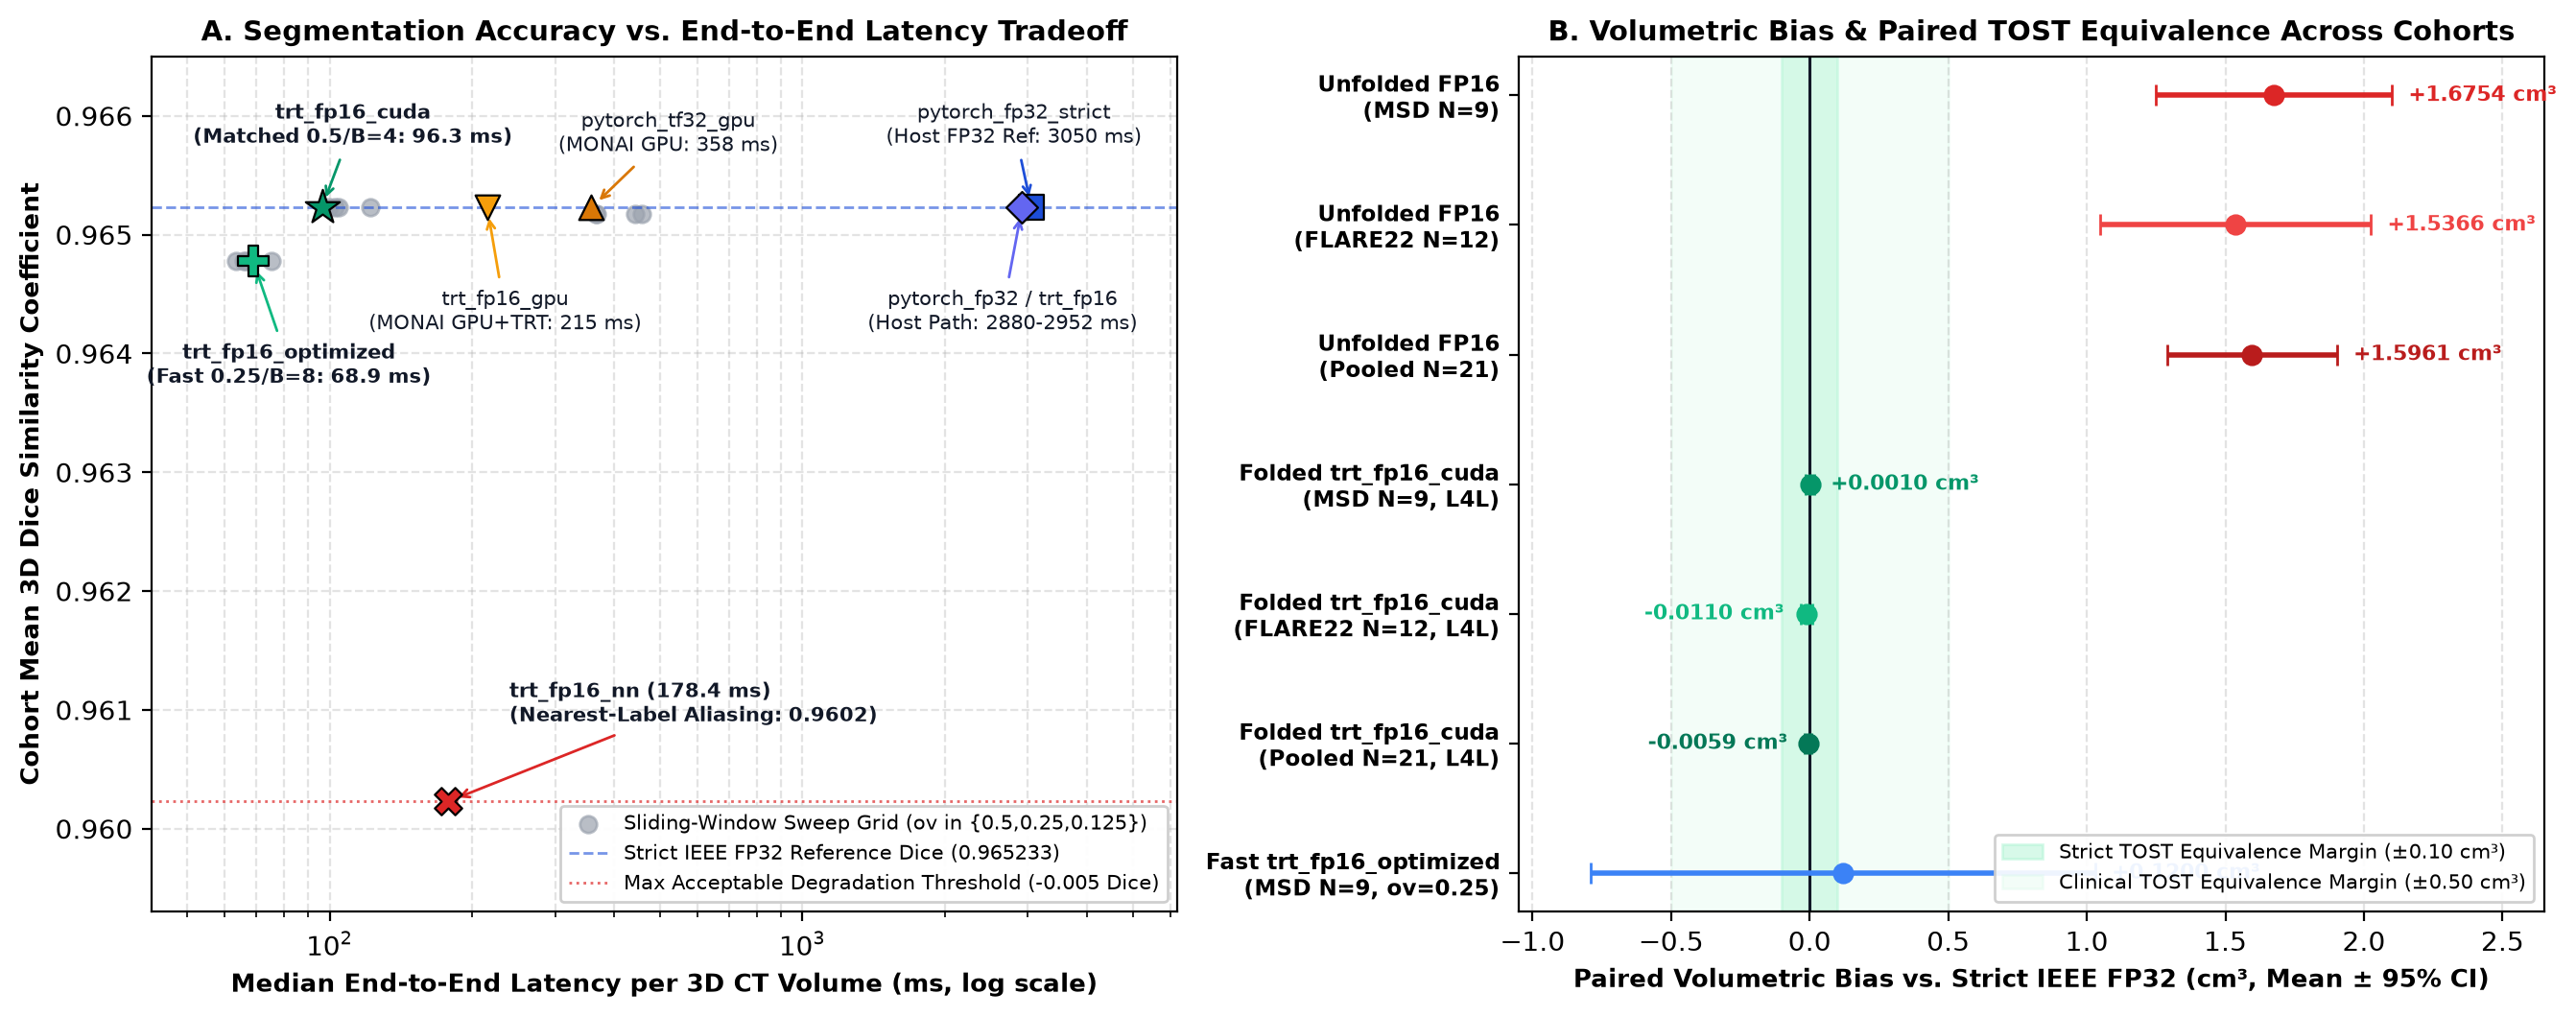
\includegraphics[width=0.88\textwidth]{figures/accuracy_vs_latency.png}\\[3pt]
    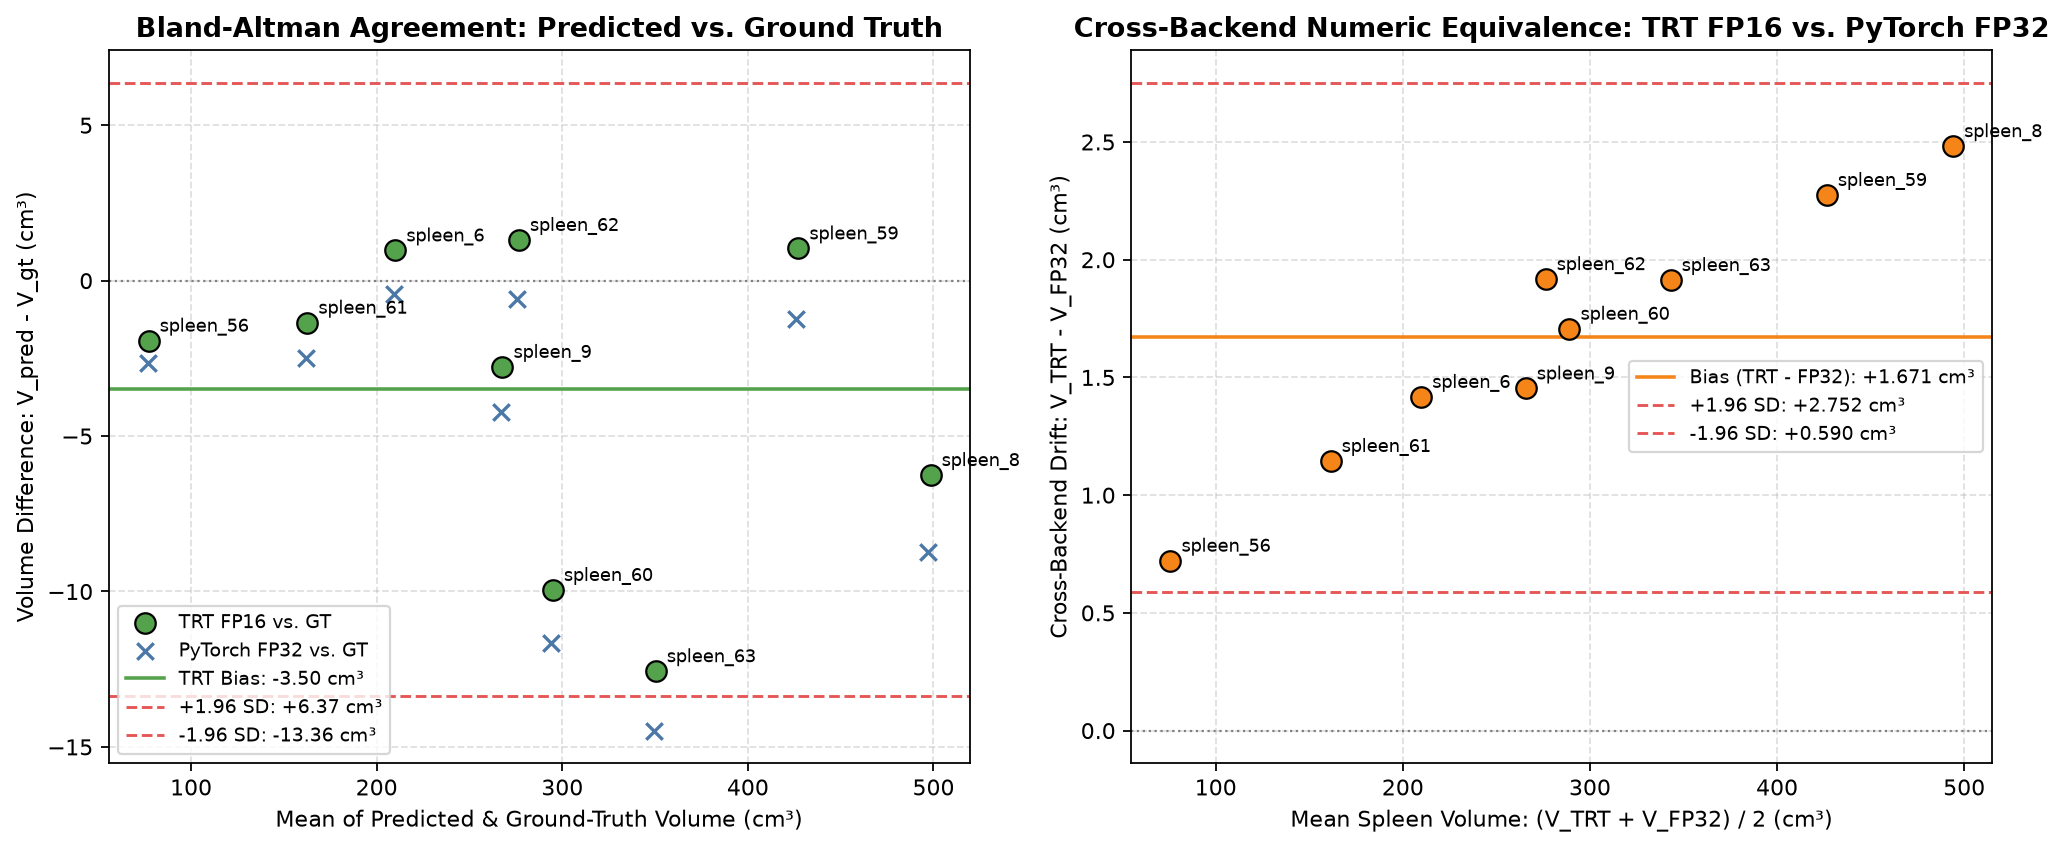
\includegraphics[width=0.31\textwidth]{figures/bland_altman.png}\hfill
    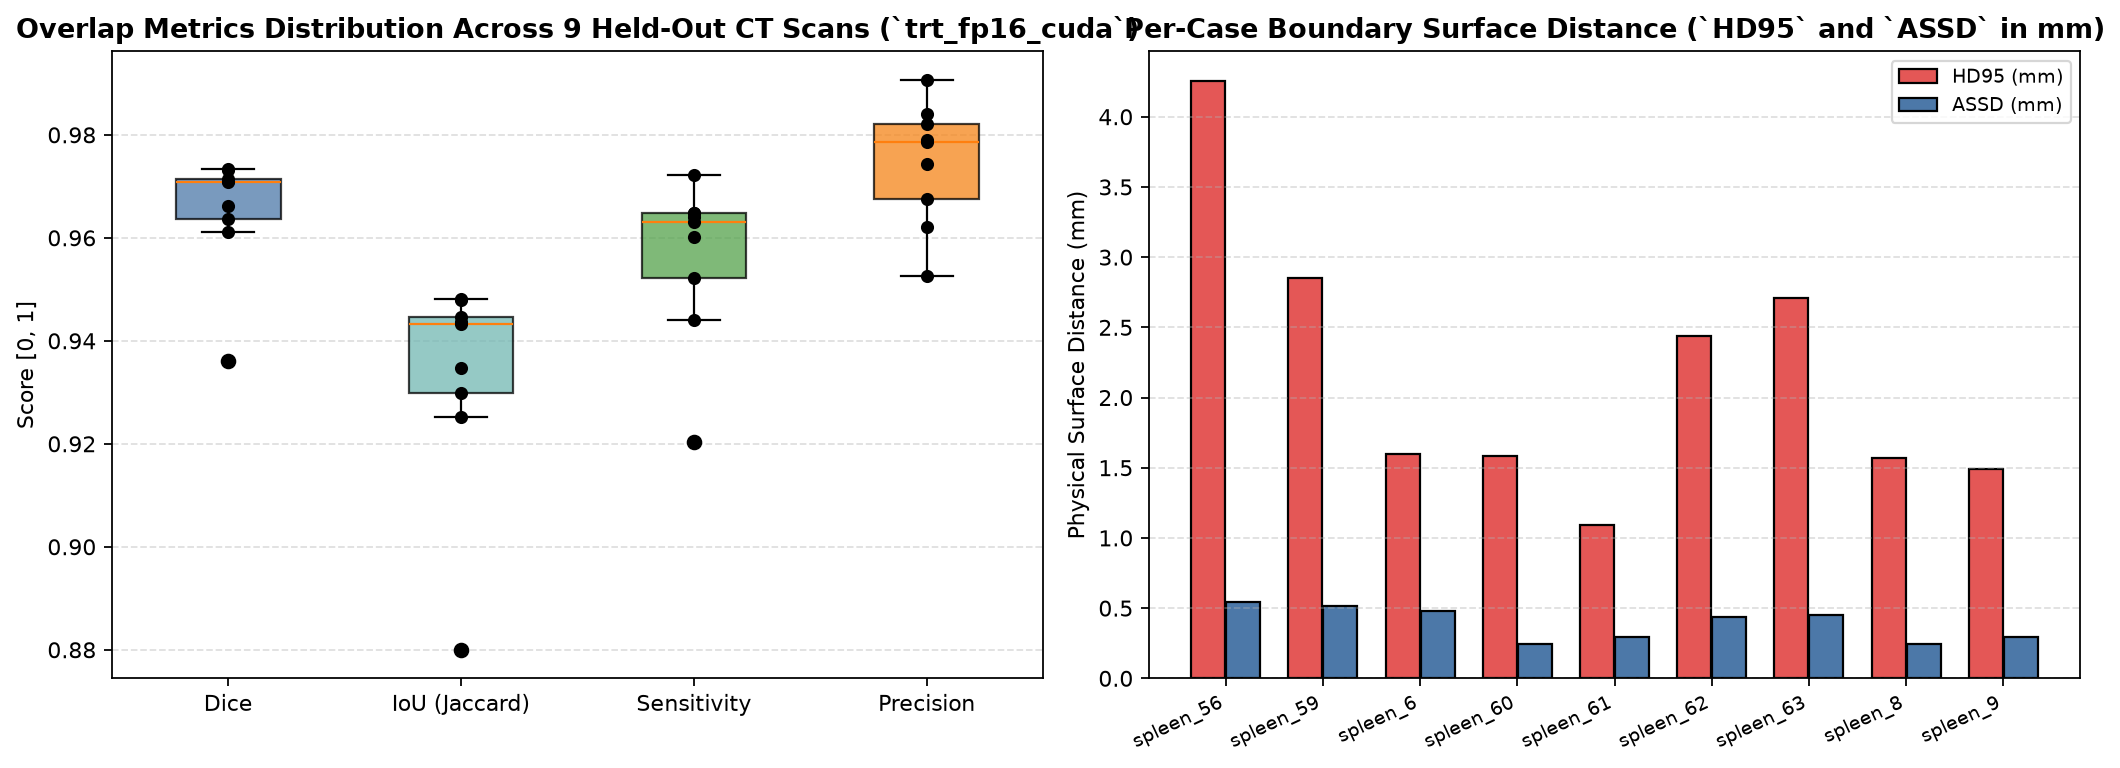
\includegraphics[width=0.31\textwidth]{figures/segmentation_metrics_distribution.png}\hfill
    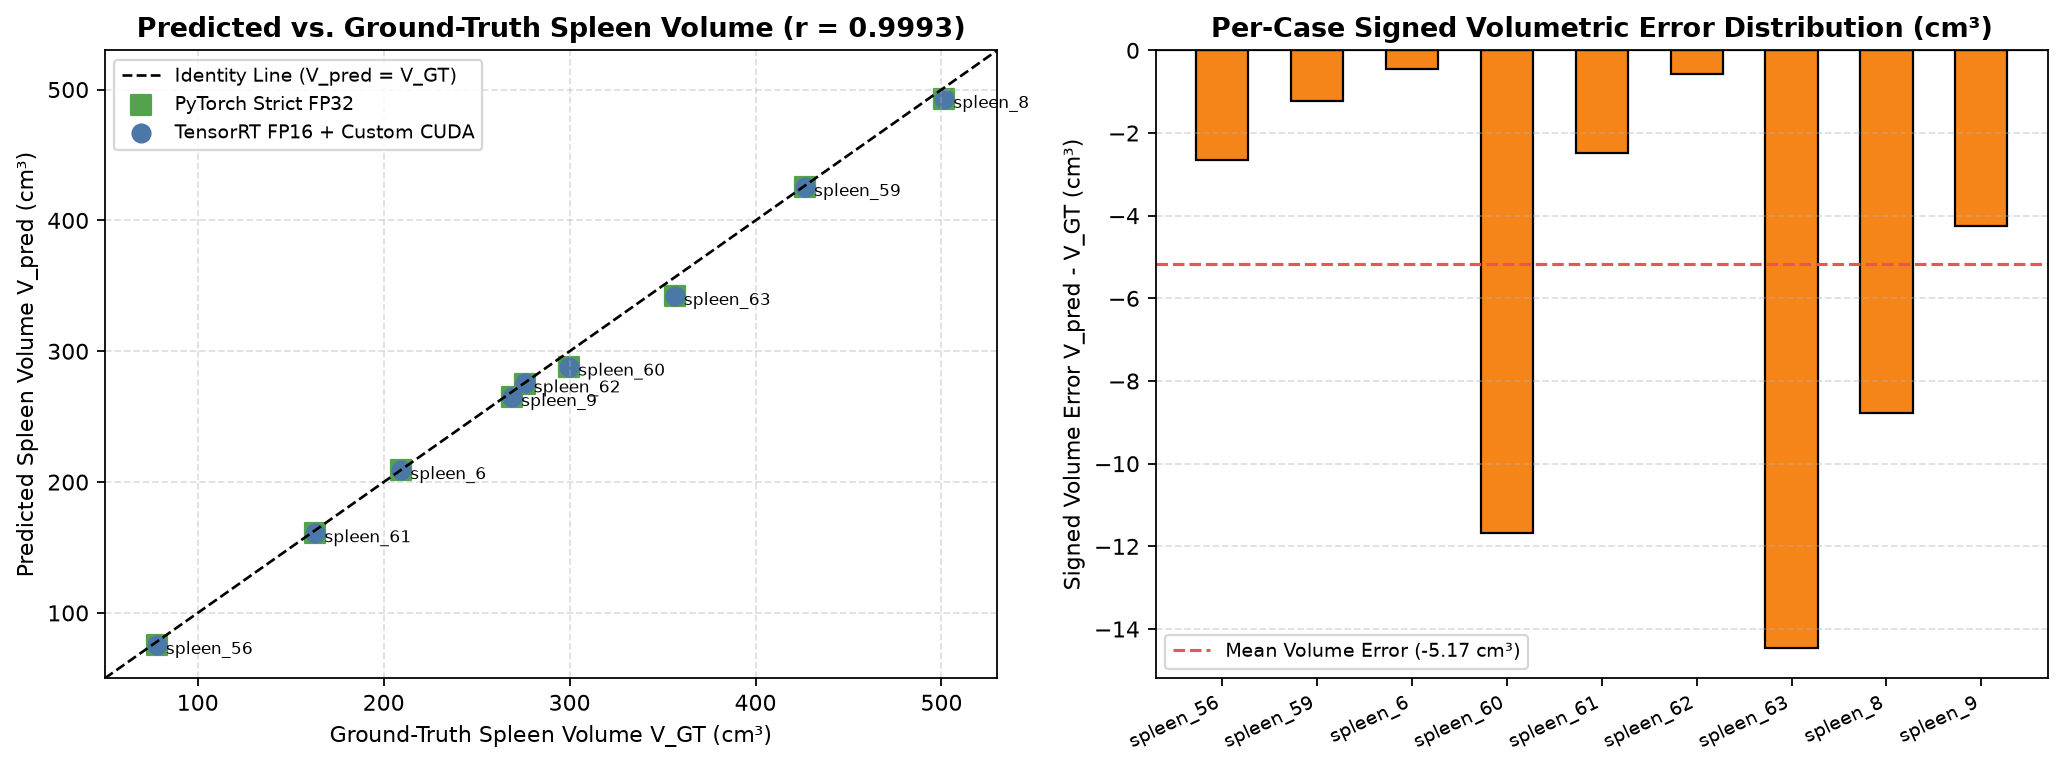
\includegraphics[width=0.31\textwidth]{figures/volumetric_scatter_and_error.png}
    \caption{\textbf{Top (A--B):} Mean 3D Dice vs.\ end-to-end latency across execution profiles and paired volumetric bias vs.\ strict IEEE FP32 ($\text{cm}^3$, Mean $\pm 95\%$ CI) against the $\pm 0.10\text{ cm}^3$ and $\pm 0.50\text{ cm}^3$ TOST equivalence regions. \textbf{Bottom:} Dual Bland--Altman volumetric agreement against strict IEEE FP32 (left), multi-metric overlap/surface distributions (center), and physical volume parity scatter (right).}
    \label{fig:tradeoff_ba}
\end{figure*}

\begin{table*}[t]
\centering
\caption{Per-patient paired latency and numerical equivalence across all $N = 9$ internal MSD validation scans and $N = 12$ external unseen MICCAI \texttt{FLARE22} scans. $\Delta V_{\text{unf}}$ and $\Delta V_{\text{cuda}}$ denote physical volume bias ($\text{cm}^3$) relative to strict IEEE FP32 (\texttt{pytorch\_fp32\_strict}).}
\label{tab:percase}
\resizebox{\textwidth}{!}{%
\begin{tabular}{llcccccccccccc}
\toprule
\textbf{Cohort / Case ID} & \textbf{Shape ($X \times Y \times Z$)} & \textbf{Win ($0.5/0.25$)} & \textbf{Host FP32 (ms)} & \textbf{CUDA L4L (ms)} & \textbf{Fast Opt (ms)} & \textbf{Paired Speedup (L4L / Opt)} & \textbf{Dice (FP32 Ref)} & \textbf{Dice (CUDA L4L)} & \textbf{$\Delta\text{Dice}$ (L4L)} & \textbf{$\text{HD}_{95}$ / ASSD (mm)} & \textbf{$V_{\text{GT}}$ ($\text{cm}^3$)} & \textbf{$\Delta V_{\text{unf}}$ / $\Delta V_{\text{cuda}}$ ($\text{cm}^3$)} & \textbf{Flipped Voxels (\% Organ)} \\
\midrule
\multicolumn{14}{l}{\textit{\textbf{Cohort 1: Internal Held-Out MSD \texttt{Task09\_Spleen} Validation Split ($N = 9$ independent patients, 10 timed passes/patient)}}}\\
\texttt{spleen\_56} & $512 \times 512 \times 33$ & $32 / 18$ & $1543.7$ & $47.6$ & $36.0$ & $32.46\times / 42.91\times$ & $0.936143$ & $0.936164$ & $+0.000021$ & $4.25 / 0.55$ & $78.07$ & $+0.722 / -0.003$ & $3 / 22,038$ ($0.0136\%$) \\
\texttt{spleen\_59} & $512 \times 512 \times 50$ & $72 / 50$ & $2570.3$ & $89.7$ & $71.6$ & $28.66\times / 35.88\times$ & $0.966229$ & $0.966251$ & $+0.000022$ & $2.85 / 0.52$ & $426.65$ & $+2.284 / +0.027$ & $10 / 94,040$ ($0.0106\%$) \\
\texttt{spleen\_6} & $512 \times 512 \times 135$ & $72 / 50$ & $6142.8$ & $123.4$ & $108.2$ & $49.79\times / 56.75\times$ & $0.973239$ & $0.973226$ & $-0.000013$ & $1.60 / 0.48$ & $209.52$ & $+1.426 / +0.005$ & $10 / 154,403$ ($0.0065\%$) \\
\texttt{spleen\_60} & $512 \times 512 \times 97$ & $125 / 64$ & $4936.4$ & $155.6$ & $101.8$ & $31.72\times / 48.49\times$ & $0.971020$ & $0.971015$ & $-0.000005$ & $1.59 / 0.25$ & $299.84$ & $+1.717 / -0.009$ & $11 / 91,659$ ($0.0120\%$) \\
\texttt{spleen\_61} & $512 \times 512 \times 101$ & $125 / 64$ & $5034.3$ & $162.4$ & $104.8$ & $31.00\times / 48.03\times$ & $0.971511$ & $0.971502$ & $-0.000009$ & $1.09 / 0.30$ & $163.30$ & $+1.149 / +0.003$ & $1 / 53,761$ ($0.0019\%$) \\
\texttt{spleen\_62} & $512 \times 512 \times 80$ & $64 / 27$ & $3789.9$ & $96.7$ & $70.1$ & $39.19\times / 54.07\times$ & $0.961134$ & $0.961119$ & $-0.000015$ & $2.44 / 0.43$ & $275.93$ & $+1.918 / +0.023$ & $16 / 120,578$ ($0.0133\%$) \\
\texttt{spleen\_63} & $512 \times 512 \times 60$ & $75 / 32$ & $2952.0$ & $98.4$ & $63.3$ & $30.01\times / 46.64\times$ & $0.963625$ & $0.963618$ & $-0.000007$ & $2.71 / 0.45$ & $356.60$ & $+1.920 / +0.011$ & $12 / 121,013$ ($0.0099\%$) \\
\texttt{spleen\_8} & $512 \times 512 \times 31$ & $50 / 32$ & $1625.1$ & $62.1$ & $47.9$ & $26.19\times / 33.92\times$ & $0.973413$ & $0.973384$ & $-0.000029$ & $1.57 / 0.24$ & $501.55$ & $+2.488 / -0.037$ & $10 / 106,587$ ($0.0094\%$) \\
\texttt{spleen\_9} & $512 \times 512 \times 41$ & $50 / 32$ & $1949.7$ & $66.7$ & $52.5$ & $29.24\times / 37.13\times$ & $0.970787$ & $0.970786$ & $-0.000001$ & $1.49 / 0.30$ & $269.15$ & $+1.456 / -0.011$ & $6 / 95,683$ ($0.0063\%$) \\
\textbf{MSD Mean $\pm$ SD} & \textit{9 Patients} & $73.9 / 41.0$ & $3393.8 \pm 1699$ & $100.3 \pm 40.3$ & $72.9 \pm 26.5$ & $\mathbf{33.14\times} / \mathbf{44.87\times}$ & $0.965233$ & $\mathbf{0.965229}$ & $-0.000004$ & $\mathbf{2.18 / 0.39}$ & $286.73$ & $\mathbf{+1.675 / +0.001}$ & $\mathbf{8.8}$ ($\mathbf{0.0093\%}$) \\
\midrule
\multicolumn{14}{l}{\textit{\textbf{Cohort 2: External Unseen Multi-Center MICCAI \texttt{FLARE22} Cohort ($N = 12$ independent patients)}}}\\
\texttt{FLARE22\_Tr\_0001} & $512 \times 512 \times 110$ & $32 / 18$ & $6367.5$ & $257.9$ & $243.3$ & $24.69\times / 26.18\times$ & $0.961213$ & $0.961207$ & $-0.000006$ & $2.32 / 0.56$ & $186.17$ & $+0.987 / -0.002$ & $16 / 175,548$ ($0.0091\%$) \\
\texttt{FLARE22\_Tr\_0002} & $512 \times 512 \times 107$ & $50 / 32$ & $5912.2$ & $276.2$ & $241.3$ & $21.40\times / 24.50\times$ & $0.964399$ & $0.964395$ & $-0.000004$ & $2.50 / 0.56$ & $281.25$ & $+1.436 / -0.010$ & $17 / 198,142$ ($0.0086\%$) \\
\texttt{FLARE22\_Tr\_0003} & $512 \times 512 \times 101$ & $50 / 32$ & $5327.0$ & $253.6$ & $236.9$ & $21.01\times / 22.49\times$ & $0.955464$ & $0.955433$ & $-0.000031$ & $2.17 / 0.66$ & $163.03$ & $+0.795 / +0.007$ & $13 / 107,077$ ($0.0121\%$) \\
\texttt{FLARE22\_Tr\_0004} & $512 \times 512 \times 87$ & $50 / 32$ & $4679.4$ & $232.9$ & $198.5$ & $20.09\times / 23.58\times$ & $0.960944$ & $0.960946$ & $+0.000002$ & $2.32 / 0.54$ & $222.10$ & $+1.171 / -0.001$ & $15 / 164,121$ ($0.0091\%$) \\
\texttt{FLARE22\_Tr\_0005} & $512 \times 512 \times 85$ & $50 / 32$ & $4915.9$ & $221.5$ & $206.5$ & $22.19\times / 23.81\times$ & $0.962419$ & $0.962391$ & $-0.000028$ & $2.45 / 0.52$ & $189.61$ & $+1.114 / +0.002$ & $13 / 122,226$ ($0.0106\%$) \\
\texttt{FLARE22\_Tr\_0006} & $512 \times 512 \times 93$ & $72 / 32$ & $5596.4$ & $263.3$ & $222.6$ & $21.26\times / 25.14\times$ & $0.960910$ & $0.960888$ & $-0.000022$ & $2.44 / 0.59$ & $174.83$ & $+0.941 / -0.004$ & $12 / 91,579$ ($0.0131\%$) \\
\texttt{FLARE22\_Tr\_0007} & $512 \times 512 \times 105$ & $50 / 32$ & $6092.1$ & $257.9$ & $247.3$ & $23.62\times / 24.64\times$ & $0.845178$ & $0.845134$ & $-0.000044$ & $20.00 / 2.87$ & $481.72$ & $+2.913 / -0.035$ & $52 / 229,102$ ($0.0227\%$) \\
\texttt{FLARE22\_Tr\_0008} & $512 \times 512 \times 99$ & $50 / 32$ & $5821.1$ & $265.6$ & $207.2$ & $21.91\times / 28.10\times$ & $0.958981$ & $0.958978$ & $-0.000003$ & $2.21 / 0.57$ & $244.87$ & $+1.395 / -0.002$ & $15 / 157,108$ ($0.0095\%$) \\
\texttt{FLARE22\_Tr\_0009} & $512 \times 512 \times 87$ & $50 / 32$ & $4878.4$ & $231.1$ & $220.9$ & $21.11\times / 22.08\times$ & $0.828880$ & $0.828552$ & $-0.000328$ & $10.95 / 2.14$ & $146.54$ & $+3.200 / -0.104$ & $80 / 65,505$ ($0.1221\%$) \\
\texttt{FLARE22\_Tr\_0010} & $512 \times 512 \times 96$ & $50 / 32$ & $5168.0$ & $251.6$ & $197.9$ & $20.54\times / 26.11\times$ & $0.966501$ & $0.966511$ & $+0.000010$ & $1.83 / 0.58$ & $367.51$ & $+1.829 / +0.010$ & $8 / 209,759$ ($0.0038\%$) \\
\texttt{FLARE22\_Tr\_0011} & $512 \times 512 \times 84$ & $50 / 32$ & $4422.4$ & $229.0$ & $204.2$ & $19.31\times / 21.66\times$ & $0.962932$ & $0.962930$ & $-0.000002$ & $2.30 / 0.58$ & $292.36$ & $+1.561 / +0.007$ & $15 / 189,184$ ($0.0079\%$) \\
\texttt{FLARE22\_Tr\_0012} & $512 \times 512 \times 103$ & $50 / 32$ & $5596.1$ & $265.1$ & $241.1$ & $21.11\times / 23.21\times$ & $0.904354$ & $0.904320$ & $-0.000034$ & $23.44 / 1.95$ & $130.75$ & $+1.099 / -0.002$ & $15 / 73,200$ ($0.0205\%$) \\
\textbf{FLARE22 Mean $\pm$ SD} & \textit{12 Patients} & $50.3 / 30.8$ & $5398.0 \pm 601$ & $250.5 \pm 17.5$ & $222.3 \pm 19.0$ & $\mathbf{21.52\times} / \mathbf{24.29\times}$ & $0.936015$ & $\mathbf{0.935974}$ & $-0.000041$ & $\mathbf{6.25 / 1.01}$ & $240.06$ & $\mathbf{+1.537 / -0.011}$ & $\mathbf{22.6}$ ($\mathbf{0.0208\%}$) \\
\bottomrule
\end{tabular}%
}
\end{table*}

\begin{table*}[t]
\centering
\caption{Formal paired Two One-Sided Tests (TOST) equivalence analysis against strict IEEE FP32 (\texttt{pytorch\_fp32\_strict}) at significance level $\alpha = 0.05$ across Internal MSD ($N=9$), External \texttt{FLARE22} ($N=12$), and Pooled ($N=21$) patient cohorts.}
\label{tab:tost}
\resizebox{\textwidth}{!}{%
\begin{tabular}{llcccccc}
\toprule
\textbf{Cohort ($N$ Patients)} & \textbf{Comparison vs.\ Strict FP32} & \textbf{Margin $\pm \Delta$} & \textbf{Mean Diff $\pm$ SD} & \textbf{90\% CI (TOST Bounds)} & \textbf{95\% CI} & \textbf{$p_{\text{TOST}}$} & \textbf{Equivalent?} \\
\midrule
MSD Internal ($N = 9$) & \texttt{trt\_fp16\_unfolded} Volume & $\pm 0.50\text{ cm}^3$ & $+1.6754 \pm 0.5531\text{ cm}^3$ & $[+1.3326, +2.0183]\text{ cm}^3$ & $[+1.2503, +2.1006]\text{ cm}^3$ & $0.9999$ & \textbf{No (Fails)} \\
MSD Internal ($N = 9$) & \textbf{\texttt{trt\_fp16\_cuda} (Folded) Volume} & $\mathbf{\pm 0.10\textbf{ cm}^3}$ & $\mathbf{+0.0010 \pm 0.0194\textbf{ cm}^3}$ & $\mathbf{[-0.0110, +0.0130]\textbf{ cm}^3}$ & $[-0.0139, +0.0159]\text{ cm}^3$ & $\mathbf{< 10^{-6}}$ & \textbf{Yes (Pass)} \\
MSD Internal ($N = 9$) & \textbf{\texttt{trt\_fp16\_cuda} (Folded) Dice} & $\mathbf{\pm 0.0010}$ & $\mathbf{-0.000004 \pm 0.000016}$ & $\mathbf{[-0.000014, +0.000006]}$ & $[-0.000017, +0.000009]$ & $\mathbf{< 10^{-6}}$ & \textbf{Yes (Pass)} \\
\midrule
FLARE22 External ($N = 12$) & \texttt{trt\_fp16\_unfolded} Volume & $\pm 0.50\text{ cm}^3$ & $+1.5366 \pm 0.7680\text{ cm}^3$ & $[+1.1385, +1.9348]\text{ cm}^3$ & $[+1.0487, +2.0246]\text{ cm}^3$ & $0.9997$ & \textbf{No (Fails)} \\
FLARE22 External ($N = 12$) & \textbf{\texttt{trt\_fp16\_cuda} (Folded) Volume} & $\mathbf{\pm 0.10\textbf{ cm}^3}$ & $\mathbf{-0.0110 \pm 0.0315\textbf{ cm}^3}$ & $\mathbf{[-0.0274, +0.0053]\textbf{ cm}^3}$ & $[-0.0311, +0.0090]\text{ cm}^3$ & $\mathbf{< 10^{-6}}$ & \textbf{Yes (Pass)} \\
FLARE22 External ($N = 12$) & \textbf{\texttt{trt\_fp16\_cuda} (Folded) Dice} & $\mathbf{\pm 0.0010}$ & $\mathbf{-0.000041 \pm 0.000092}$ & $\mathbf{[-0.000089, +0.000007]}$ & $[-0.000099, +0.000018]$ & $\mathbf{< 10^{-6}}$ & \textbf{Yes (Pass)} \\
\midrule
\textbf{Pooled Cohorts ($N = 21$)} & \texttt{trt\_fp16\_unfolded} Volume & $\pm 0.50\text{ cm}^3$ & $+1.5961 \pm 0.6721\text{ cm}^3$ & $[+1.3432, +1.8491]\text{ cm}^3$ & $[+1.2902, +1.9021]\text{ cm}^3$ & $1.0000$ & \textbf{No (Fails)} \\
\textbf{Pooled Cohorts ($N = 21$)} & \textbf{\texttt{trt\_fp16\_cuda} (Folded) Volume} & $\mathbf{\pm 0.10\textbf{ cm}^3}$ & $\mathbf{-0.0059 \pm 0.0271\textbf{ cm}^3}$ & $\mathbf{[-0.0161, +0.0043]\textbf{ cm}^3}$ & $[-0.0182, +0.0064]\text{ cm}^3$ & $\mathbf{< 10^{-6}}$ & \textbf{Yes (Pass)} \\
\textbf{Pooled Cohorts ($N = 21$)} & \textbf{\texttt{trt\_fp16\_cuda} (Folded) Dice} & $\mathbf{\pm 0.0010}$ & $\mathbf{-0.000025 \pm 0.000071}$ & $\mathbf{[-0.000052, +0.000002]}$ & $[-0.000058, +0.000007]$ & $\mathbf{< 10^{-6}}$ & \textbf{Yes (Pass)} \\
\bottomrule
\end{tabular}%
}
\end{table*}

\section{Discussion and Broader Implications}
\label{sec:discussion}

\subsection{Interactive 3D Segmentation Workstations and Cohort Screening}
Compressing end-to-end 3D CT segmentation latency from $2.95\text{--}6.14\text{ s}$ to $68.9\text{--}96.3\text{ ms}$ ($10.4\text{--}14.5\text{ volumes/s}$) transforms volumetric organ segmentation from an offline batch job into an interactive operation suitable for research review workstations (\texttt{app/workstation.py}) and retrospective multi-thousand-scan imaging studies.

\subsection{Numerical Conditioning as a Prerequisite for Reduced-Precision Medical AI}
Our diagnosis of the $+1.68\text{ cm}^3$ (MSD) and $+1.54\text{ cm}^3$ (\texttt{FLARE22}) unfolded FP16 volume dilation demonstrates that aggregate overlap scores alone (Dice $0.9657$ vs.\ $0.9652$) fail to detect systematic directional bias in reduced-precision inference. In quantitative longitudinal studies measuring organ volume change across serial scans, a $+1.6\text{ cm}^3$ software bias introduced solely by switching from an FP32 PyTorch checkpoint to an unfused FP16 TensorRT engine would confound biological effect sizes. Pre-export algebraic conditioning in IEEE-754 \texttt{float64} removes this bias at zero runtime overhead.

\subsection{Register-Level Spatial Computing and High-Density GPU Co-Residency}
Replacing MONAI's $2,301\text{ MB}$ \texttt{float64} coordinate meshgrids with scalar register-computed $3 \times 4$ affine transformations ($455\text{ MB}$ peak VRAM) enables five concurrent 3D segmentation pipelines to co-reside inside the memory budget previously occupied by a single transform call. More generally, MedTRT illustrates three transferable HPC design principles: (1) Amdahl-guided full-pipeline profiling before kernel specialization, (2) substituting $O(1)$ per-thread scalar register arithmetic for $O(D \cdot H \cdot W \cdot 3)$ global memory traffic, and (3) exact pre-compilation conditioning of ill-scaled normalization layers.

\section{Limitations and Scope Boundaries}
\label{sec:limitations}

To uphold strict scientific transparency, we document nine scope boundaries:
\begin{enumerate}
    \item \textbf{Internal Checkpoint Split ($N=9$) \& External Sample Size ($N=12$):} The 9 internal MSD validation scans had zero overlap with gradient training, but upstream MONAI checkpoint selection evaluated validation Dice on those 9 scans because official MSD \texttt{imagesTs} labels are unannotated. Our 12 external multi-center \texttt{FLARE22} scans ($N=21$ pooled patients, $53$ total CT volumes) provide an independent unseen cohort, though broader clinical characterization requires $N > 100$ multi-institutional studies.
    \item \textbf{Single-Organ Binary Architecture:} Experiments evaluate a binary 3D Residual U-Net segmenting the spleen; multi-organ architectures ($13\text{--}104$ classes) require multi-channel top-$K$ postprocessing.
    \item \textbf{Single Modality:} Benchmarks evaluate abdominal CT with fixed HU windowing rather than multi-sequence MRI or PET/CT.
    \item \textbf{Single Laptop GPU under Windows WDDM:} Timings reflect an NVIDIA RTX 5080 Laptop GPU (\texttt{sm\_120}, $90\text{ W}$ TGP) under Windows 11 WDDM scheduling; absolute latencies differ on Linux TCC datacenter GPUs or embedded Jetson modules.
    \item \textbf{Warm Page-Cache vs.\ Cold Storage \& Decompression:} Primary GPU benchmarks measure pre-decompressed \texttt{.nii} files in warm OS page cache ($29.2\text{ ms}$ ingest; $23.8\text{ ms}$ cold unbuffered NVMe read vs.\ $175.4\text{ ms}$ over virtualized cloud storage), excluding one-time \texttt{.nii.gz} decompression ($265.0\text{ ms}$ standalone).
    \item \textbf{Steady-State Process Timing:} Benchmarks exclude one-time Python startup, CUDA initialization, NVRTC compilation, and TensorRT engine deserialization.
    \item \textbf{Local File Ingestion:} Hospital DICOM network association and series assembly are outside repository scope.
    \item \textbf{Single-Stream Execution:} Latency reflects sequential single-volume execution rather than multi-client batching.
    \item \textbf{Non-Clinical Research Prototype:} MedTRT is an educational and research engineering study and is not a cleared medical device.
\end{enumerate}

\section{Future Research Directions}
\label{sec:future}

Future extensions target eight directions: (A) \textbf{Multi-Organ Sparse Interpolation:} generalizing \texttt{fused\_invert\_trilinear\_threshold\_u8} to top-$K$ probability channels for 13-organ \texttt{FLARE} and 104-structure \texttt{TotalSegmentator} models; (B) \textbf{Multi-Modality Kernels:} register-fused $z$-score normalization for 3D MRI and PET/CT; (C) \textbf{Blackwell FP8 \& Calibrated INT8:} pairing analytical BatchNorm folding with native \texttt{FP8} (\texttt{E4M3}) Tensor Core execution; (D) \textbf{CUDA Graph Capture:} encapsulating all sliding-window launches inside a single \texttt{cudaGraphExec\_t}; (E) \textbf{TensorRT \texttt{IPluginV3} Integration:} embedding register-affine CUDA kernels directly inside serialized \texttt{.engine} plans; (F) \textbf{Dual-Stream DMA Overlapping:} pipelining PCIe \texttt{h2d} transfer of volume $i+1$ with inference on volume $i$; (G) \textbf{Embedded Edge Profiling:} benchmarking power-constrained throughput on NVIDIA Jetson Orin/Thor modules; and (H) \textbf{Asynchronous Pinned DICOM Assembly:} streaming raw DICOM slices directly into pinned host staging buffers.

\section{Conclusion}
\label{sec:conclusions}

Order-of-magnitude end-to-end acceleration of volumetric 3D CT organ segmentation requires co-designing storage ingestion, register-level GPU spatial kernels, and numerical graph conditioning around the neural network. By replacing host \texttt{.nii.gz} decompression and MONAI's $2,301\text{ MB}$ \texttt{float64} GPU coordinate meshgrids with memory-mapped ingestion and nine custom register-affine CUDA C++17 kernels, MedTRT achieves a $\mathbf{30.67\times}$ cohort median speedup ($\mathbf{33.14\times}$ paired patient-level mean speedup at $\mathbf{96.3\textbf{ ms}}$) under controlled matched sliding windows and a $\mathbf{42.86\times}$ cohort speedup ($\mathbf{46.64\times}$ paired median at $\mathbf{68.9\textbf{ ms}}$) under fast sliding windows, while cutting peak GPU memory by $\mathbf{5.06\times}$ ($\mathbf{455\textbf{ MB}}$). Simultaneously, analytical \texttt{float64} \texttt{ConvTranspose3d+BatchNorm3d} folding resolves the $-81.79$ decoder FP16 cancellation bug, reducing logit drift by $\mathbf{35.6\times}$ and satisfying formal paired TOST equivalence ($p_{\text{TOST}} < 10^{-6}$) within $\pm 0.10\text{ cm}^3$ across $N = 21$ internal MSD and unseen external MICCAI \texttt{FLARE22} patients.

\begin{thebibliography}{99}
\footnotesize
\bibitem{kerfoot2019} E. Kerfoot \textit{et al.}, ``Left-Ventricle Quantification Using Residual U-Net,'' in \textit{STACOM 2018, LNCS}, vol. 11395, pp. 371--380, Springer, 2019.
\bibitem{cicek2016} \"O. \c{C}i\c{c}ek \textit{et al.}, ``3D U-Net: Learning Dense Volumetric Segmentation from Sparse Annotation,'' in \textit{MICCAI 2016, LNCS}, vol. 9901, pp. 424--432, 2016.
\bibitem{cardoso2022} M. J. Cardoso \textit{et al.}, ``MONAI: An open-source framework for deep learning in healthcare,'' \textit{arXiv:2211.02701}, 2022.
\bibitem{monaibundle2024} MONAI Consortium, ``MONAI Model Zoo: \texttt{spleen\_ct\_segmentation} Bundle v0.6.1,'' Apache-2.0 License, 2024. \url{https://github.com/Project-MONAI/model-zoo}
\bibitem{xia2018} Y. Xia \textit{et al.}, ``3D Semi-Supervised Learning with Uncertainty-Aware Multi-View Co-Training,'' \textit{arXiv:1811.12506}, 2018.
\bibitem{antonelli2022} M. Antonelli \textit{et al.}, ``The Medical Segmentation Decathlon,'' \textit{Nature Communications}, vol. 13, no. 1, p. 4128, 2022 (CC-BY-SA 4.0).
\bibitem{simpson2019} A. L. Simpson \textit{et al.}, ``A large annotated medical image dataset for the development and evaluation of segmentation algorithms,'' \textit{arXiv:1902.09063}, 2019.
\bibitem{ma2023flare} J. Ma \textit{et al.}, ``Fast and Low-GPU-memory Abdomen CT Organ Segmentation: The FLARE Challenge,'' \textit{Medical Image Analysis}, vol. 82, p. 102616, 2022, and Zenodo Record \texttt{7860267}, 2023.
\bibitem{amdahl1967} G. M. Amdahl, ``Validity of the single processor approach to achieving large scale computing capabilities,'' in \textit{Proc. AFIPS}, pp. 483--485, 1967.
\bibitem{paszke2019} A. Paszke \textit{et al.}, ``PyTorch: An Imperative Style, High-Performance Deep Learning Library,'' in \textit{NeurIPS}, vol. 32, pp. 8024--8035, 2019.
\bibitem{onnx2019} J. Bai \textit{et al.}, ``ONNX: Open Neural Network Exchange,'' 2019, and ONNX Runtime Developers, \url{https://onnxruntime.ai/}, 2021.
\bibitem{tensorrt2025} NVIDIA Corporation, \textit{NVIDIA TensorRT 10.16 Developer Guide \& CUDA 12.8 Runtime/Driver API Reference}, 2025.
\bibitem{nickolls2008} J. Nickolls, I. Buck, M. Garland, and K. Skadron, ``Scalable Parallel Programming with CUDA,'' \textit{ACM Queue}, vol. 6, no. 2, pp. 40--53, 2008.
\bibitem{brett2024} M. Brett \textit{et al.}, ``nipy/nibabel: 5.4.2,'' \textit{Zenodo}, 2024; C. R. Harris \textit{et al.}, ``Array programming with NumPy,'' \textit{Nature}, vol. 585, pp. 357--362, 2020; P. Virtanen \textit{et al.}, ``SciPy 1.0,'' \textit{Nature Methods}, vol. 17, pp. 261--272, 2020.
\bibitem{dice1945} L. R. Dice, ``Measures of the amount of ecologic association between species,'' \textit{Ecology}, vol. 26, no. 3, pp. 297--302, 1945.
\bibitem{taha2015} A. A. Taha and A. Hanbury, ``Metrics for evaluating 3D medical image segmentation: analysis, selection, and tool,'' \textit{BMC Medical Imaging}, vol. 15, no. 1, p. 29, 2015.
\bibitem{bland1986} J. M. Bland and D. G. Altman, ``Statistical methods for assessing agreement between two methods of clinical measurement,'' \textit{The Lancet}, vol. 327, no. 8476, pp. 307--310, 1986.
\bibitem{schuirmann1987} D. J. Schuirmann, ``A comparison of the two one-sided tests procedure and the power approach for assessing the equivalence of average bioavailability,'' \textit{Journal of Pharmacokinetics and Biopharmaceutics}, vol. 15, no. 6, pp. 657--680, 1987.
\end{thebibliography}

\end{document}
